\documentclass[conference]{IEEEtran}
\IEEEoverridecommandlockouts

% Paquetes esenciales para ingeniería
\usepackage[spanish,es-tabla]{babel}
\usepackage[utf8]{inputenc}
\usepackage{amsmath,amssymb,amsfonts}
\usepackage{graphicx}
\usepackage{siunitx}
\usepackage{booktabs}
\usepackage{pgfplots}
\usepackage{circuitikz}
\usepackage{hyperref}
\usepackage{xcolor}
\usepackage{float}
\usepackage{cite}

\pgfplotsset{compat=1.17}

\begin{document}

\title{Red Telefónica Pública Conmutada (PSTN), Simulación de Señales Analógicas y Análisis Espectral de Armónicos en MATLAB y Simulink}

\author{
    \IEEEauthorblockN{John David Ureña Meléndez\thanks{Código fuente disponible en: \url{https://github.com/Ing-jdum/COMUNICACIONES-1-INTEC/tree/main/lab/tarea2}}}
    \textit{1085857}
    \IEEEauthorblockA{\textit{Facultad de Ingeniería Eléctrica} \\
    \textit{Instituto Tecnológico de Santo Domingo (INTEC)}\\
    Asignatura: Comunicaciones \\
    Fecha: 10 de agosto de 2026}
}

\maketitle

\begin{abstract}
Este informe documenta el estudio conceptual de la Red Telefónica Pública Conmutada (PSTN) y la simulación en MATLAB y Simulink de doce señales analógicas de referencia, una señal senoidal amortiguada, y una señal eléctrica de 60~Hz con cinco armónicos superpuestos, empleada para ilustrar la Distorsión Armónica Total (THD) en sistemas de potencia y su interacción con las telecomunicaciones. Se modeló y analizó cada una de las doce señales en los dominios del tiempo y de la frecuencia mediante la Transformada Rápida de Fourier (FFT), documentando explícitamente los supuestos adoptados ante ambigüedades del enunciado en los ítems 1, 2, 7, 9 y 12. Para la señal armónica se construyó un modelo Simulink (\texttt{modelo\_armonicos\_60hz}) con seis fuentes senoidales de amplitudes 120, 60, 40, 30, 24 y 20~V en 60, 120, 180, 240, 300 y 360~Hz; el análisis espectral obtenido mediante \texttt{findpeaks} ubicó los seis picos dentro de 0.06~Hz de las frecuencias de diseño y con error de amplitud inferior al 2\%, confirmando que, para esta configuración particular ($F_s=10\,000$~Hz, ventana de 0.1~s, seis periodos exactos de la fundamental), el espectro obtenido coincide con el esperado y no exhibe aliasing ni fuga espectral apreciable. Se implementó además en LabVIEW el ejercicio de análisis espectral de la guía, mediante un VI con dos bloques \textit{Simulate Signal} (0.05~Hz/amplitud 1 y 0.25~Hz/amplitud 0.5, a $F_s=20$~S/s y $N=1024$) y bloques \textit{Spectral Measurements} en modo \textit{Power Spectrum} lineal: los espectros medidos ubicaron sendos picos en 0.05 y 0.25~Hz con magnitudes de 0.39 y 0.12 respectivamente, para una resolución espectral $\Delta f = F_s/N \approx 0.0195$~Hz; la suma de ambas señales antes del análisis produjo un espectro con las dos líneas independientes e inalteradas, verificando experimentalmente la linealidad de la Transformada de Fourier, mientras que el escenario de submuestreo propuesto en la guía (0.3~S/s) resultó irrealizable porque el propio Express VI rechaza toda tasa inferior al doble de la frecuencia de la señal, y la mínima tasa admitida (0.5~S/s, exactamente $2f$ para la componente de 0.25~Hz) anuló dicha componente hasta el nivel de residuo numérico ($\sim10^{-14}$), ilustrando por qué el criterio de Nyquist se enuncia con desigualdad estricta. Se aborda también el rol regulatorio de la FCC y la ITU en la telefonía y la asignación de espectro. Los resultados numéricos completos, doce señales analizadas, cuatro figuras de armónicos y cinco capturas del montaje en LabVIEW, permiten vincular la teoría de señales y sistemas con los mecanismos de operación de la PSTN.
\end{abstract}

\begin{IEEEkeywords}
PSTN, señales analógicas, FFT, armónicos, THD, muestreo de Nyquist, Simulink.
\end{IEEEkeywords}

\section{Introducción}

La Red Telefónica Pública Conmutada (\textit{Public Switched Telephone Network}, PSTN) constituye la infraestructura de conmutación de circuitos que, durante más de un siglo, ha soportado la comunicación de voz a nivel mundial, y cuyos principios de diseño (ancho de banda de voz limitado a 4~kHz, jerarquía de centrales de conmutación, planes de numeración normalizados) siguen influyendo en la arquitectura de las redes de telecomunicaciones modernas, incluso a medida que estas migran hacia esquemas de conmutación de paquetes. Comprender la PSTN exige, a su vez, comprender el comportamiento de las señales analógicas que la atraviesan: su forma en el dominio del tiempo, su contenido espectral, y los mecanismos por los cuales el muestreo, la distorsión armónica y el ruido afectan la fidelidad de la información transmitida.

Este informe aborda ambos aspectos. En primer lugar, se sintetiza el marco conceptual de la PSTN a partir del material de la asignatura: sus componentes físicos, la jerarquía de centrales, el plan de numeración NPA-NXX-Station, y su evolución hacia redes de próxima generación (NGN). En segundo lugar, se documenta un conjunto de simulaciones en MATLAB y Simulink orientadas a reforzar, mediante la práctica, los conceptos de muestreo, transformada de Fourier y análisis armónico: la generación y el análisis temporal/espectral de doce señales analógicas de referencia y una señal senoidal amortiguada, y la simulación de una señal eléctrica de 60~Hz distorsionada por cinco armónicos adicionales, representativa de las cargas no lineales que introducen ruido armónico tanto en redes eléctricas como en líneas de comunicación adyacentes. Se incluye además la implementación y ejecución en LabVIEW del ejercicio de análisis espectral propuesto en la guía, con sus capturas del diagrama de bloques y del panel frontal, y un breve tratamiento de los organismos reguladores (FCC, ITU) y de los principales tipos de cableado empleados en redes de telecomunicaciones y datos.

\section{Objetivos}

\subsection{Objetivo General}
Analizar los fundamentos de la Red Telefónica Pública Conmutada y comprender, mediante simulación en MATLAB y Simulink, el comportamiento temporal y espectral de señales analógicas de referencia y de señales eléctricas con contenido armónico.

\subsection{Objetivos Específicos}
\begin{itemize}
    \item Describir los componentes físicos y la jerarquía de conmutación de la PSTN, así como su plan de numeración y su evolución hacia redes de próxima generación.
    \item Generar y graficar en MATLAB doce señales analógicas de referencia (funciones trigonométricas, exponenciales, exponenciales complejas, escalón, tren de pulsos, funciones tipo \textit{Sa}/sinc, secuencia discreta, diente de sierra y superposición de senoidales) en los dominios del tiempo y de la frecuencia.
    \item Interpretar físicamente cada señal generada y relacionarla con fenómenos reales de telecomunicaciones (muestreo, modulación, transitorios de conmutación, señalización digital, barridos de frecuencia, distorsión armónica).
    \item Simular una señal senoidal amortiguada representativa de la respuesta transitoria de un sistema de segundo orden.
    \item Modelar en MATLAB y Simulink una señal eléctrica de 60~Hz compuesta por una fundamental y cinco armónicos, calculando su Distorsión Armónica Total (THD) y analizando su espectro mediante FFT.
    \item Comparar los resultados espectrales obtenidos en Simulink con los valores de diseño, evaluando la presencia de aliasing, fuga espectral o errores de resolución.
    \item Implementar en LabVIEW el ejercicio de análisis espectral propuesto en la guía, verificando experimentalmente la resolución espectral, la relación entre amplitud temporal y magnitud espectral, la linealidad de la Transformada de Fourier y las consecuencias de muestrear en el límite del criterio de Nyquist.
    \item Explicar el rol regulatorio de la FCC y la ITU, y describir brevemente los principales tipos de cableado utilizados en redes de telecomunicaciones y datos.
\end{itemize}

\section{Marco Teórico}

\subsection{La Red Telefónica Pública Conmutada (PSTN)}

La PSTN es una red de conmutación de circuitos compuesta, en su forma clásica, por cuatro elementos principales: las centrales telefónicas (\textit{switches}), la red de señalización (históricamente el sistema de señalización por canal común número 7, SS7), la red de interconexión troncal entre centrales, y el bucle de abonado o \textit{local loop}, el par de cobre que conecta al equipo terminal del cliente (\textit{Customer Premises Equipment}, CPE, por ejemplo un teléfono o un módem) con la central local más cercana \cite{itu-q23}. Las centrales se organizan históricamente en una jerarquía de cuatro niveles, central local (conecta directamente a los abonados), central primaria, central secundaria y central terciaria o de tránsito, de modo que una llamada entre abonados distantes se enruta ascendiendo por la jerarquía hasta encontrar una ruta común y descendiendo hacia el destino, minimizando así el número de enlaces de larga distancia necesarios.

El bucle de abonado transporta tradicionalmente una señal de voz analógica cuyo ancho de banda se limita, por convención internacional, a la banda de 300--3400~Hz, aproximada en el diseño de sistemas a 4~kHz al incluir una banda de guarda que facilita el filtrado anti-aliasing previo a la digitalización de la señal en la central (típicamente mediante modulación por código de pulsos, PCM, a 8000 muestras por segundo). Esta limitación de ancho de banda, heredada del diseño original de la red analógica, es la razón por la cual esquemas de señalización como DTMF (estudiado en la Tarea 1 de esta asignatura) emplean frecuencias dentro de dicha banda vocal.

La identificación de cada abonado dentro de la PSTN se realiza mediante un plan de numeración jerárquico. En Norteamérica y el Caribe (incluyendo República Dominicana), el \textit{North American Numbering Plan} (NANP) estructura cada número telefónico en tres campos: el código de área o \textit{Numbering Plan Area} (NPA, tres dígitos), el código de intercambio o central (NXX, tres dígitos, donde el segundo dígito no puede ser 9 y ciertas combinaciones están reservadas) y el número de estación (\textit{Station}, cuatro dígitos). Por ejemplo, el número \texttt{234-234-5678} es una asignación válida bajo este esquema (NPA=234, NXX=234, Station=5678), mientras que \texttt{123-234-5678} es inválido porque ningún código de área NPA puede comenzar con el dígito 1, reservado como prefijo de acceso a llamada de larga distancia dentro del NANP.

\subsection{Evolución hacia redes de próxima generación}

La PSTN tradicional, basada en conmutación de circuitos dedicados durante toda la duración de la llamada, ha evolucionado progresivamente hacia las redes de próxima generación (\textit{Next Generation Networks}, NGN), en las que la función de conmutación de circuitos es reemplazada por un \textit{softswitch}, un elemento de control implementado en software que separa el plano de señalización del plano de transporte, y la voz se transporta como paquetes digitales (por ejemplo, mediante Voz sobre IP) sobre una red de conmutación de paquetes común a otros servicios de datos, en lugar de un circuito dedicado por llamada. Esta convergencia reduce el costo de infraestructura, al compartir una única red de transporte para voz, datos y video, pero introduce nuevos retos de calidad de servicio (latencia, \textit{jitter}, pérdida de paquetes) ausentes en la conmutación de circuitos original, donde el ancho de banda estaba garantizado durante toda la llamada.

\subsection{Muestreo, Fourier y resolución espectral}

Toda señal analógica de ancho de banda limitado $f_{max}$ puede reconstruirse exactamente a partir de sus muestras si la frecuencia de muestreo satisface el criterio de Nyquist-Shannon, $F_s > 2 f_{max}$ \cite{oppenheim}. El análisis espectral de una señal discreta de $N$ muestras se realiza habitualmente mediante la Transformada Rápida de Fourier (FFT), cuya resolución en frecuencia está dada por
\begin{equation}
\Delta f = \frac{1}{T} = \frac{F_s}{N}
\label{eq:resolucion}
\end{equation}
donde $T=N/F_s$ es la duración de la ventana de observación \cite{oppenheim}. Componentes espectrales separadas por menos de $\Delta f$ no pueden distinguirse con certeza en el espectro resultante, y ventanas de observación que no contienen un número entero de periodos de la señal producen fuga espectral (\textit{spectral leakage}), fenómeno por el cual la energía de una componente pura se dispersa hacia contenedores de frecuencia (\textit{bins}) vecinos \cite{proakis}.

\subsection{Armónicos y distorsión armónica total}

En un sistema eléctrico ideal, la tensión y la corriente son senoidales puras a la frecuencia fundamental de la red (60~Hz en el sistema dominicano y norteamericano). Las cargas no lineales (rectificadores, variadores de frecuencia, fuentes conmutadas, balastros electrónicos) inyectan corrientes con componentes en múltiplos enteros de la fundamental, los armónicos, que se superponen a la fundamental y deforman la onda senoidal original \cite{proakis}. La Distorsión Armónica Total (THD) cuantifica esta deformación como la razón entre el valor eficaz (RMS) de todos los armónicos, excluyendo la fundamental, y el valor eficaz de la fundamental:
\begin{equation}
\text{THD} = \frac{\sqrt{\sum_{k=2}^{\infty} A_k^2}}{A_1}
\label{eq:thd}
\end{equation}
donde $A_k$ es la amplitud del armónico de orden $k$. Un THD elevado se traduce en sobrecalentamiento de conductores y transformadores por pérdidas adicionales (efecto piel, corrientes de Foucault), en interferencia electromagnética hacia equipos de comunicación cercanos, y en errores de medición en instrumentos que asumen una forma de onda puramente senoidal, razón por la cual normas como IEEE 519 limitan el THD admisible en instalaciones eléctricas.

\section{Desarrollo Experimental}

\subsection{Herramientas y organización de los scripts}

Las simulaciones se realizaron en MATLAB, complementadas con un modelo construido programáticamente en Simulink y con un VI desarrollado en LabVIEW (\texttt{Tarea2.vi}, dentro del proyecto \texttt{Tarea 2.lvproj}) para el ejercicio de análisis espectral descrito en la Sección VIII. Se emplearon tres scripts principales:
\begin{itemize}
    \item Un script para el Ejercicio 1, que genera y grafica las doce señales analógicas de referencia (ítems 1 a 12 del enunciado) y la señal senoidal amortiguada complementaria, calculando en cada caso la señal continua, su versión discretizada (\texttt{stem}) y su espectro de magnitud y fase mediante FFT.
    \item Un script para el Ejercicio 3, que genera los seis armónicos de una señal eléctrica de 60~Hz, la señal suma resultante y su espectro FFT.
    \item Un script complementario que construye programáticamente el modelo Simulink \texttt{modelo\_armonicos\_60hz}, ejecuta la simulación y exporta la señal muestreada a MATLAB para su análisis temporal y espectral, dado que los bloques \textit{Scope} y \textit{Spectrum Analyzer} de Simulink no pueden capturarse como imagen en modo de ejecución \texttt{-batch} (sin interfaz gráfica).
\end{itemize}

\subsection{Supuestos documentados ante ambigüedades del enunciado}

El enunciado del Ejercicio 1 presenta varias expresiones cuya interpretación matemática no es única. Los supuestos adoptados, documentados en el sidecar de notas del script, se listan a continuación:
\begin{itemize}
    \item \textbf{Ítem 1:} la expresión ``1-sen(2xt)'' se interpretó como $x_1(t) = 1 - \sin(2Xt)$, es decir, la resta entre la constante 1 y la función seno, con $X=2$ multiplicando el argumento del seno y no la amplitud.
    \item \textbf{Ítem 2:} la función $\text{Sa}(2Xt)$ con $X=2.4$ se implementó mediante la función \texttt{sinc} normalizada de MATLAB ($\text{sinc}(u)=\sin(\pi u)/(\pi u)$), dividiendo el argumento entre $\pi$ para recuperar la función de muestreo clásica $\text{Sa}(u)=\sin(u)/u$ requerida por el enunciado.
    \item \textbf{Ítem 7:} el enunciado especifica $X=2j$ (un valor complejo) para la señal $-5\sin(5t)\,e^{3.5t}$, pero dicha fórmula ya es de valor real y no ofrece una posición natural donde insertar una escala compleja sin contradecir la expresión dada. Se optó por graficar la expresión literal sin aplicar $X$, documentando explícitamente esta ambigüedad en lugar de forzar una interpretación arbitraria.
    \item \textbf{Ítem 9:} la función $\sin(2t)/(2t)$ se implementó de forma manual (no mediante \texttt{sinc} de MATLAB) para dejar explícito el manejo de la indeterminación en $t=0$, fijando $x_9(0)=1$ mediante el límite de L'Hôpital, tal como sugiere el enunciado al presentar la expresión sin normalizar por $\pi$.
    \item \textbf{Ítem 12:} la amplitud $A$ de las señales $Y_1=A\sin(5\omega t)$ y $Y_2=1.2A\sin(4\omega t)$ no está especificada en el enunciado; se asumió $A=1$ como amplitud de referencia unitaria, mientras que $f=100$~Hz y $\omega=2\pi f$ se tomaron directamente del enunciado.
\end{itemize}
Los ítems restantes (3, 4, 5, 6, 8, 10, 11) se implementaron de forma directa siguiendo la fórmula y la constante $X$ indicadas explícitamente en el enunciado, sin ambigüedad relevante.

\subsection{Parámetros de simulación}

La Tabla \ref{tab:parametros_ej1} resume los parámetros generales del Ejercicio 1, y la Tabla \ref{tab:parametros_ej3} los del Ejercicio 3 (armónicos de 60~Hz) y su contraparte en Simulink.

\begin{table}[!t]
\centering
\caption{Parámetros generales del Ejercicio 1 (señales analógicas)}
\label{tab:parametros_ej1}
\begin{tabular}{|l|c|}
\hline
\textbf{Parámetro} & \textbf{Valor} \\ \hline
Vector de tiempo base & $t=0$:$0.001$:$2$ s \\ \hline
Vector de tiempo, ítem 11 (sawtooth) & $t=0$:$0.001$:$15$ s \\ \hline
Frecuencia de muestreo implícita & 1000 Hz \\ \hline
Zero-padding FFT, ítem 10 (discreto) & 64 puntos \\ \hline
Señal amortiguada: $t$ & $0$:$0.1$:$30$ s \\ \hline
Señal amortiguada: rango graficado & $[0,35]$ s, $[-1,1]$ \\ \hline
\end{tabular}
\end{table}

\begin{table}[!t]
\centering
\caption{Parámetros del Ejercicio 3 (armónicos de 60 Hz) y modelo Simulink}
\label{tab:parametros_ej3}
\begin{tabular}{|l|c|}
\hline
\textbf{Parámetro} & \textbf{Valor} \\ \hline
Frecuencia fundamental & 60 Hz \\ \hline
Amplitudes $A_1$--$A_6$ & 120, 60, 40, 30, 24, 20 V \\ \hline
Frecuencias armónicas & 60, 120, 180, 240, 300, 360 Hz \\ \hline
Ventana de análisis (MATLAB, FFT) & $t=0$:$0.001$:$0.1$ s ($F_s{=}1000$ Hz) \\ \hline
$F_s$ del solver Simulink & 10\,000 Hz ($T_s=10^{-4}$ s) \\ \hline
Tiempo de simulación Simulink & 0.100 s \\ \hline
Muestras registradas ($N$) & 1001 \\ \hline
Resolución espectral Simulink & $F_s/N = 9.990$ Hz \\ \hline
\end{tabular}
\end{table}

\subsection{Modelo Simulink \texttt{modelo\_armonicos\_60hz}}

El modelo se construyó con seis bloques \textit{Sine Wave} independientes, uno por cada componente armónica (amplitudes y frecuencias de la Tabla \ref{tab:parametros_ej3}), conectados a un bloque \textit{Add} (\texttt{Suma\_armonicos}) de seis entradas que produce la señal eléctrica distorsionada. La salida del sumador se bifurca hacia un bloque \textit{Scope} para visualización en el dominio del tiempo, un bloque \textit{Spectrum Analyzer} (condicionado a la disponibilidad de la \textit{DSP System Toolbox}) para visualización espectral en tiempo real, y un bloque \textit{To Workspace} que exporta la señal muestreada (variable \texttt{ysum\_simulink}) para su posterior análisis en MATLAB, dado que los \textit{scopes} de Simulink no pueden capturarse como imagen en una ejecución \texttt{-batch}. El solver se configuró a paso fijo con $T_s = 10^{-4}$~s ($F_s=10\,000$~Hz) y tiempo de simulación de 0.100~s.

\section{Resultados: Ejercicio 1 (Señales Analógicas)}

Esta sección analiza cada una de las doce señales del enunciado en dos fases: (Fase 1) qué representa físicamente la señal, distinguiendo entre cantidades físicas reales (voltaje, corriente) y funciones matemáticas abstractas sin correspondencia física directa; y (Fase 2) su interpretación técnica, es decir, dónde aparece un fenómeno equivalente en telecomunicaciones y cómo afecta la calidad de la señal transmitida.

\subsection{Ítem 1: $x_1(t) = 1-\sin(2Xt)$, $X=2$}
\textbf{Fase 1.} Es una función matemática abstracta (no representa directamente un voltaje o corriente física), consistente en una senoidal desplazada verticalmente en 1 unidad y con frecuencia angular escalada por $X$. \textbf{Fase 2.} El desplazamiento de nivel de continua (DC) sobre una portadora senoidal es análogo al offset de polarización que se añade a una señal de información antes de transmitirla sobre un medio que no admite valores negativos (por ejemplo, ciertos esquemas de modulación de intensidad óptica); un offset mal calibrado desperdicia margen dinámico del canal.

\subsection{Ítem 2: $x_2(t) = \text{Sa}(2Xt)$, $X=2.4$}
\textbf{Fase 1.} Es la función de muestreo (\textit{sampling function}), una función matemática sin magnitud física directa, pero de enorme relevancia teórica. \textbf{Fase 2.} La función $\text{Sa}(u)=\sin(u)/u$ es la transformada de Fourier de un pulso rectangular ideal y, recíprocamente, el filtro de reconstrucción ideal (filtro pasa-bajas ideal) en el dominio del tiempo tiene esta forma; por ello, es la función central en el teorema de muestreo de Nyquist-Shannon. Sus lóbulos laterales, que decaen lentamente, son la causa matemática de la interferencia intersímbolo (ISI) cuando un sistema de comunicación digital no emplea un filtro conformador de pulso con decaimiento más rápido (por ejemplo, coseno realzado) en lugar de un $\text{sinc}$ puro. La Figura \ref{fig:item2} muestra la señal y su espectro, donde se aprecia el carácter tipo pulso rectangular de este último.

\begin{figure}[!t]
\centering
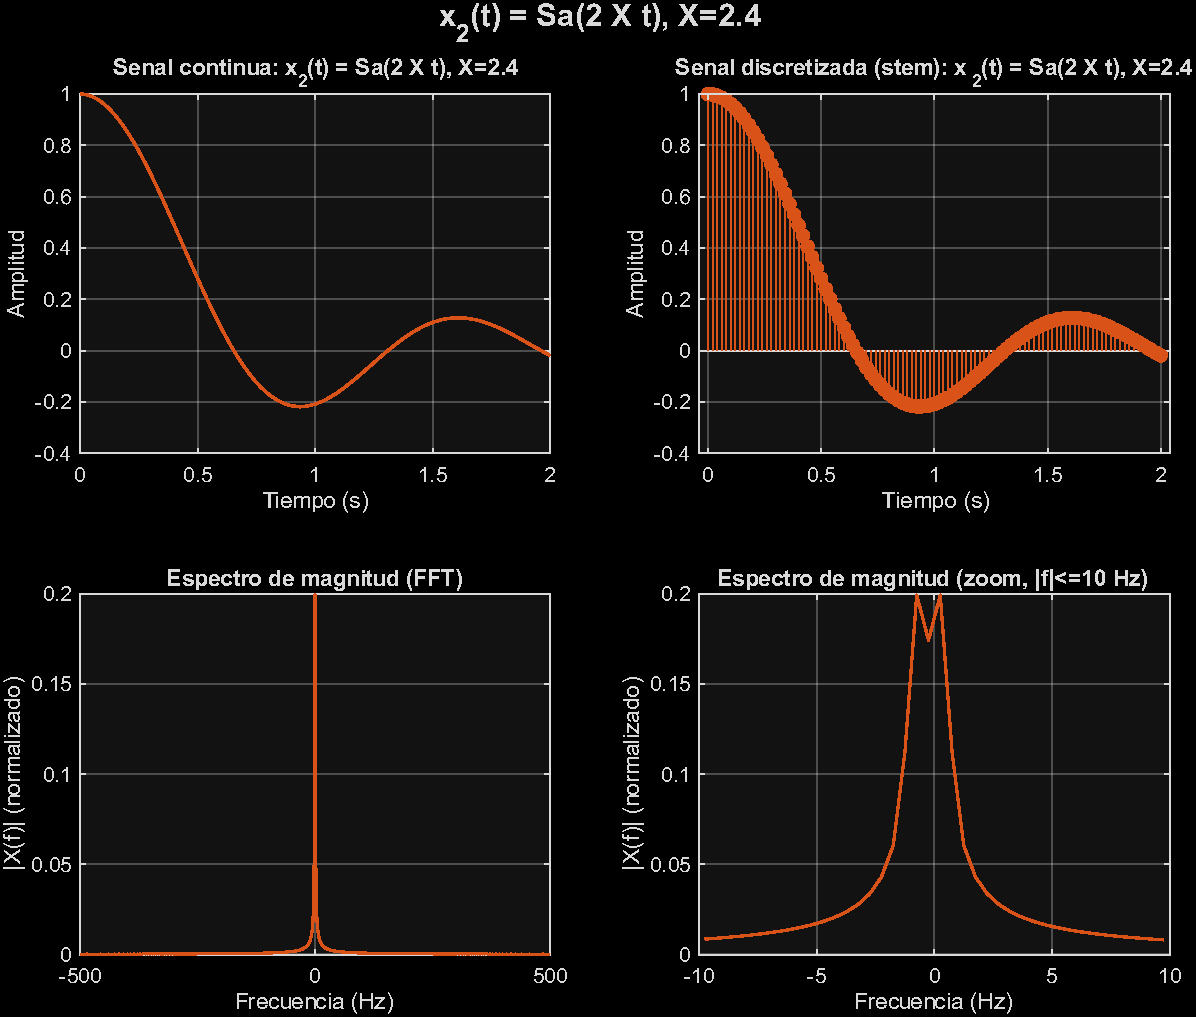
\includegraphics[width=\columnwidth]{images/01_item02_Sa.pdf}
\caption{Ítem 2: función de muestreo $x_2(t)=\text{Sa}(2Xt)$, $X=2.4$. Señal continua, versión discretizada, magnitud y acercamiento del espectro FFT.}
\label{fig:item2}
\end{figure}

\subsection{Ítem 3: $x_3(t) = \text{Re}\{Xe^{-jt}\}$, $X=3$}
\textbf{Fase 1.} Es una función matemática abstracta que, algebraicamente, se reduce a $x_3(t)=3\cos(t)$, una senoidal pura; en un circuito real podría representar un voltaje o corriente. \textbf{Fase 2.} La representación como parte real de una exponencial compleja es la notación fasorial estándar en el análisis de circuitos de corriente alterna y en el procesamiento de señales de banda base equivalente (\textit{complex baseband}) empleada en receptores de radiofrecuencia modernos, donde la señal real transmitida se recupera como la parte real de una envolvente compleja multiplicada por una portadora.

\subsection{Ítem 4: $x_4(t) = \text{Im}\{Xe^{-jt}\}$, $X=3$}
\textbf{Fase 1.} Análogamente al ítem anterior, se reduce algebraicamente a $x_4(t)=-3\sin(t)$. \textbf{Fase 2.} La parte imaginaria de la misma exponencial compleja corresponde, en el mismo esquema de banda base equivalente, a la componente en cuadratura (Q) de un modulador o demodulador I/Q, empleado en prácticamente todos los sistemas de comunicación digital moderna (QAM, QPSK) para transmitir dos flujos de información independientes sobre la misma portadora.

\subsection{Ítem 5: escalón unitario $u(t)$}
\textbf{Fase 1.} Es una función matemática idealizada; ninguna señal física real presenta una transición instantánea, aunque se aproxima razonablemente bien mediante transitorios de conmutación rápidos. \textbf{Fase 2.} El escalón modela el cierre o apertura abrupta de un circuito, como el momento en que un abonado descuelga el auricular (\textit{off-hook}) y cierra el bucle de corriente continua que la central telefónica detecta para iniciar el procesamiento de la llamada; su espectro de banda infinita implica que cualquier transición abrupta real introduce energía de alta frecuencia (ruido impulsivo/de conmutación) que debe filtrarse para no interferir con canales adyacentes. La Figura \ref{fig:item5} muestra el salto y su espectro.

\begin{figure}[!t]
\centering
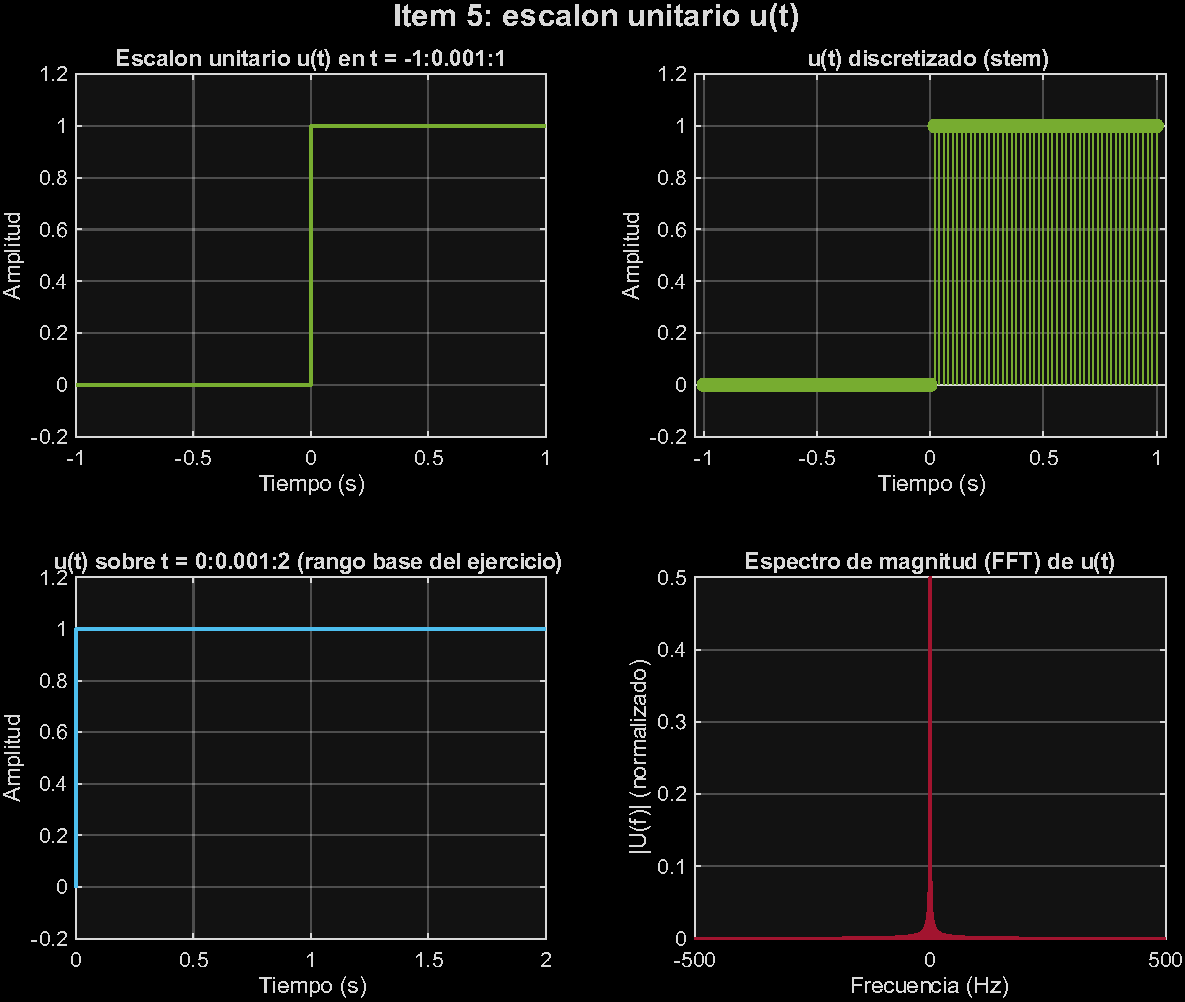
\includegraphics[width=\columnwidth]{images/01_item05_escalon.pdf}
\caption{Ítem 5: escalón unitario $u(t)$, mostrado en un rango simétrico para apreciar el salto, su versión discretizada sobre el rango base del ejercicio y su espectro de magnitud.}
\label{fig:item5}
\end{figure}

\subsection{Ítem 6: tren de pulsos cuadrados $\pm5$~V, periodo 1~s}
\textbf{Fase 1.} Representa directamente una cantidad física, un voltaje que alterna entre $+5$~V y $-5$~V. \textbf{Fase 2.} La onda cuadrada es el modelo idealizado de una señal digital binaria en banda base (NRZ, \textit{Non-Return-to-Zero}), como la empleada en la señalización de línea de módems antiguos o en buses digitales de baja velocidad; su descomposición en armónicos impares de amplitud decreciente ($1, 1/3, 1/5,\dots$) explica por qué un canal de ancho de banda limitado deforma sus bordes (redondeando las transiciones abruptas), fenómeno directamente relacionado con la limitación de ancho de banda del bucle de abonado analógico de 4~kHz. La Figura \ref{fig:item6} muestra las dos oscilaciones completas simuladas.

\begin{figure}[!t]
\centering
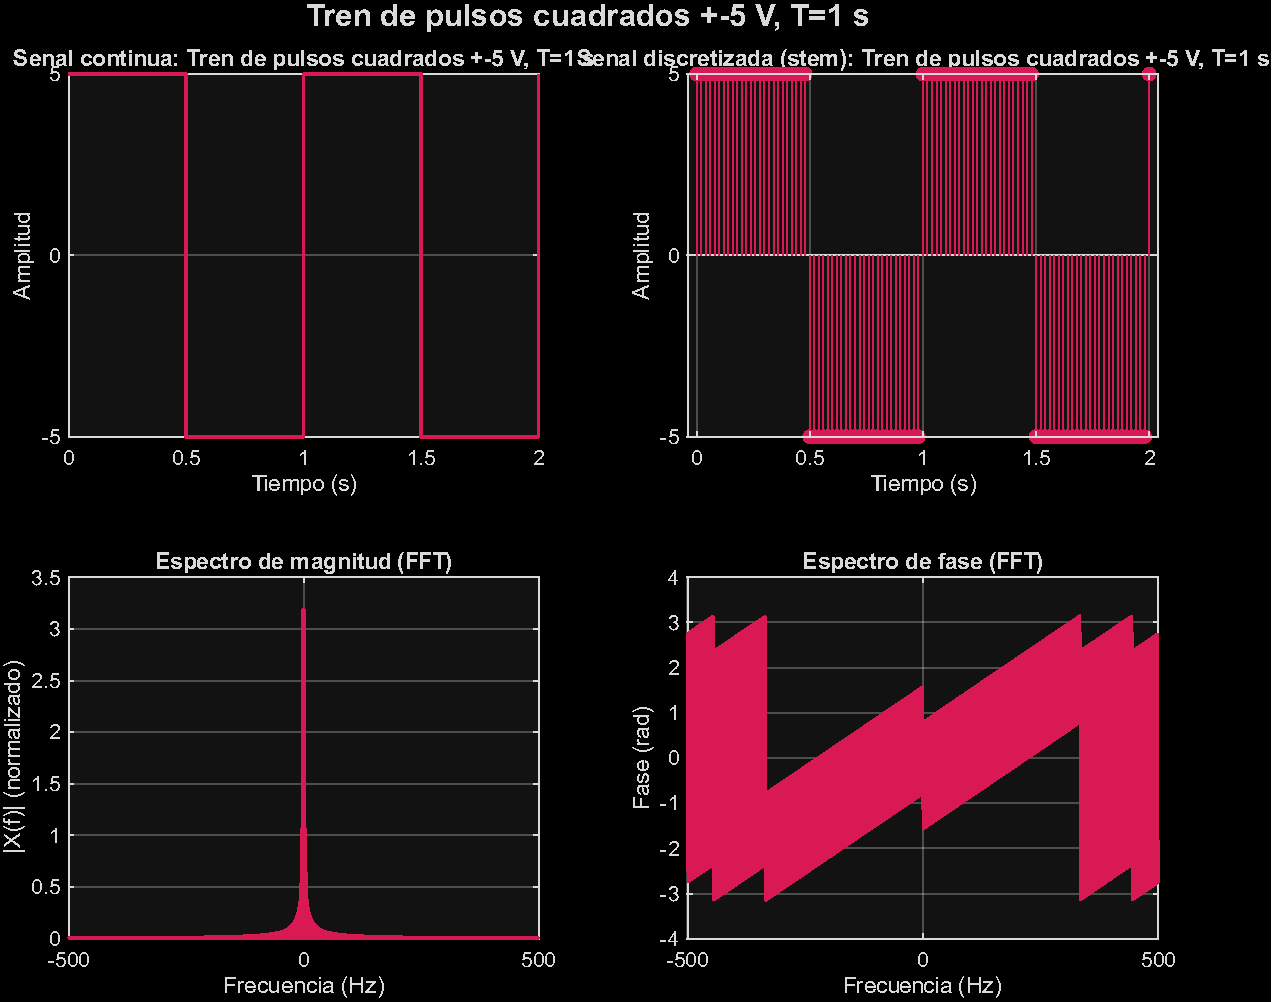
\includegraphics[width=\columnwidth]{images/01_item06_cuadrada.pdf}
\caption{Ítem 6: tren de pulsos cuadrados $\pm5$~V, periodo 1~s (frecuencia fundamental 1~Hz), señal continua, discretizada y espectro FFT.}
\label{fig:item6}
\end{figure}

\subsection{Ítem 7: $x_7(t) = -5\sin(5t)\,e^{3.5t}$}
\textbf{Fase 1.} Es una función matemática abstracta de amplitud creciente sin cota; no representa una señal física sostenible (ningún sistema real puede crecer exponencialmente sin límite), aunque aproxima el comportamiento transitorio de un sistema inestable en un intervalo acotado. \textbf{Fase 2.} Un seno modulado por una exponencial creciente es el modelo clásico de un oscilador con retroalimentación positiva neta (sistema inestable), como el que se produce en un enlace con acoplamiento acústico excesivo entre micrófono y altavoz (efecto Larsen/realimentación acústica) o en un amplificador con ganancia de lazo mayor a la unidad; en telecomunicaciones, este comportamiento se evita mediante control automático de ganancia y análisis de estabilidad de polos. La Figura \ref{fig:item7} muestra el crecimiento de la envolvente dentro del intervalo simulado.

\begin{figure}[!t]
\centering
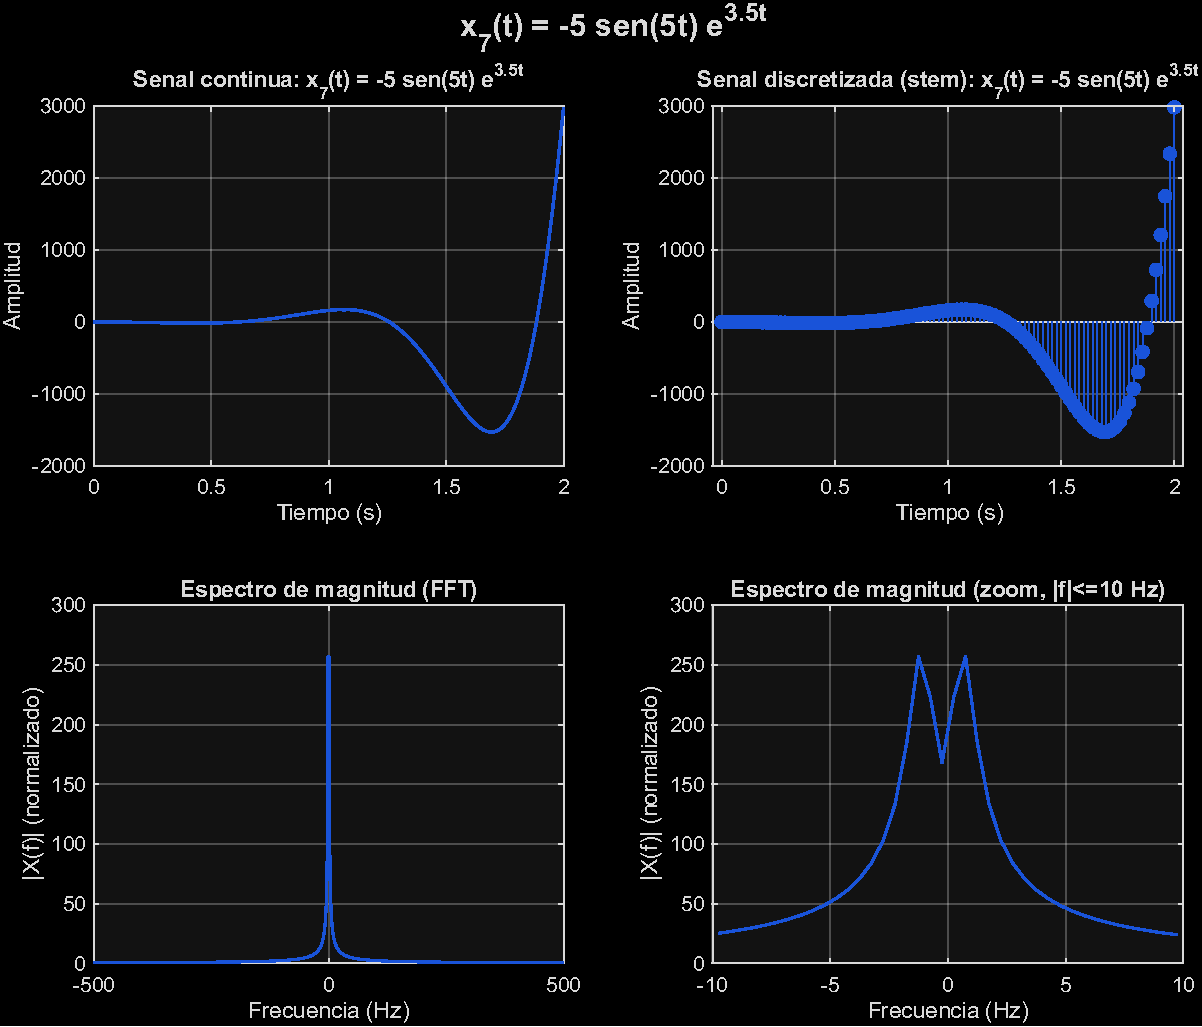
\includegraphics[width=\columnwidth]{images/01_item07_exp_creciente.pdf}
\caption{Ítem 7: $x_7(t)=-5\sin(5t)e^{3.5t}$, señal de amplitud creciente. Señal continua, discretizada y magnitud del espectro (acercamiento en bajas frecuencias por el ensanchamiento causado por el crecimiento exponencial).}
\label{fig:item7}
\end{figure}

\subsection{Ítem 8: $x_8(t) = X|\cos(2t)e^{-jt}|$, $X=1.5$}
\textbf{Fase 1.} Dado que $|e^{-jt}|=1$ para todo $t$ real, la expresión se reduce algebraicamente a $x_8(t)=1.5|\cos(2t)|$, una función matemática de valor siempre no negativo. \textbf{Fase 2.} La operación de valor absoluto sobre una senoidal es el modelo básico de un rectificador de onda completa, el circuito empleado en la etapa de alimentación de equipos de telecomunicaciones para convertir corriente alterna en corriente continua; espectralmente, la rectificación duplica la frecuencia aparente de la señal y genera una componente de continua más armónicos pares, mecanismo directamente relacionado con la generación de armónicos estudiada en la Sección VI.

\subsection{Ítem 9: $x_9(t) = \sin(2t)/(2t)$}
\textbf{Fase 1.} Es la misma familia de función matemática de muestreo que el ítem 2, aquí sin escalamiento adicional del argumento y con la indeterminación en $t=0$ resuelta por el límite $x_9(0)=1$. \textbf{Fase 2.} Refuerza la misma interpretación técnica del ítem 2: esta función es, en esencia, la respuesta al impulso de un filtro pasa-bajas ideal y aparece de forma recurrente en el análisis del teorema de muestreo, en la interpolación de señales muestreadas (reconstrucción \textit{sinc}) y en el diseño de filtros conformadores de pulso, donde su decaimiento lento en el tiempo (lóbulos laterales) debe truncarse o suavizarse para hacerlo realizable, a costa de introducir cierta ISI residual. La Figura \ref{fig:item9} ilustra su forma característica.

\begin{figure}[!t]
\centering
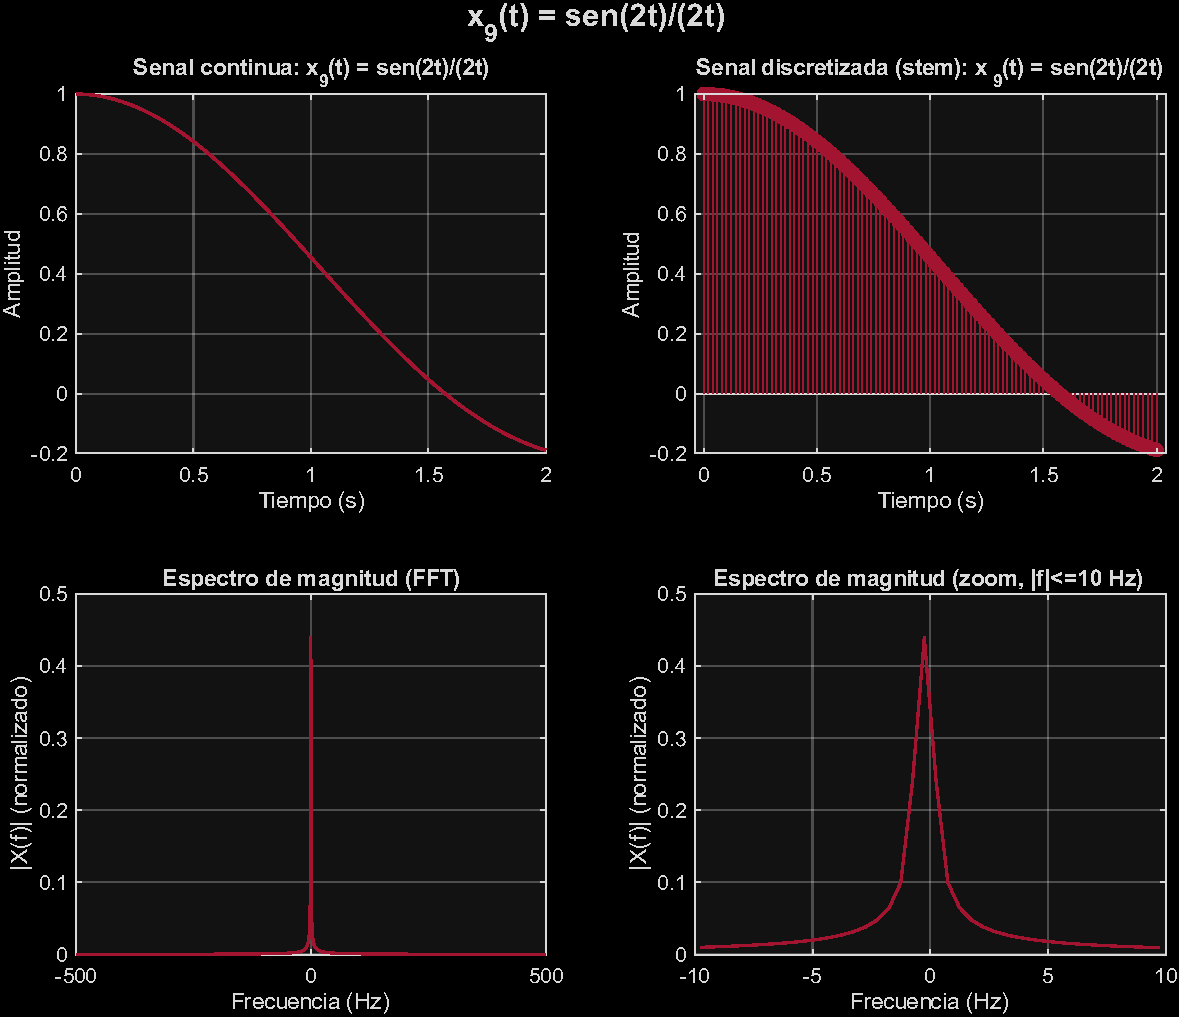
\includegraphics[width=\columnwidth]{images/01_item09_sinc_manual.pdf}
\caption{Ítem 9: $x_9(t)=\sin(2t)/(2t)$ con $x_9(0)=1$ por L'Hôpital. Señal continua, discretizada y espectro FFT.}
\label{fig:item9}
\end{figure}

\subsection{Ítem 10: secuencia discreta $x[n]$}
\textbf{Fase 1.} Es, por construcción, una secuencia de tiempo discreto pura ($x[0]=2$, $x[1]=1$, resto 0); no existe una versión de tiempo continuo subyacente, por lo que se trata honestamente como lo que es: una función matemática abstracta sin correspondencia con una cantidad física continua, mostrada únicamente mediante \texttt{stem} y su FFT con \textit{zero-padding} a 64 puntos. \textbf{Fase 2.} Secuencias discretas de este tipo son el modelo directo de los símbolos digitales en un sistema de comunicación digital (por ejemplo, los coeficientes de un filtro FIR o una secuencia de entrenamiento/preámbulo); su FFT revela el contenido espectral que dicha secuencia impone sobre la señal transmitida, información esencial para el diseño de filtros digitales en receptores de telecomunicaciones. La Figura \ref{fig:item10} muestra la secuencia y su espectro con \textit{zero-padding}.

\begin{figure}[!t]
\centering
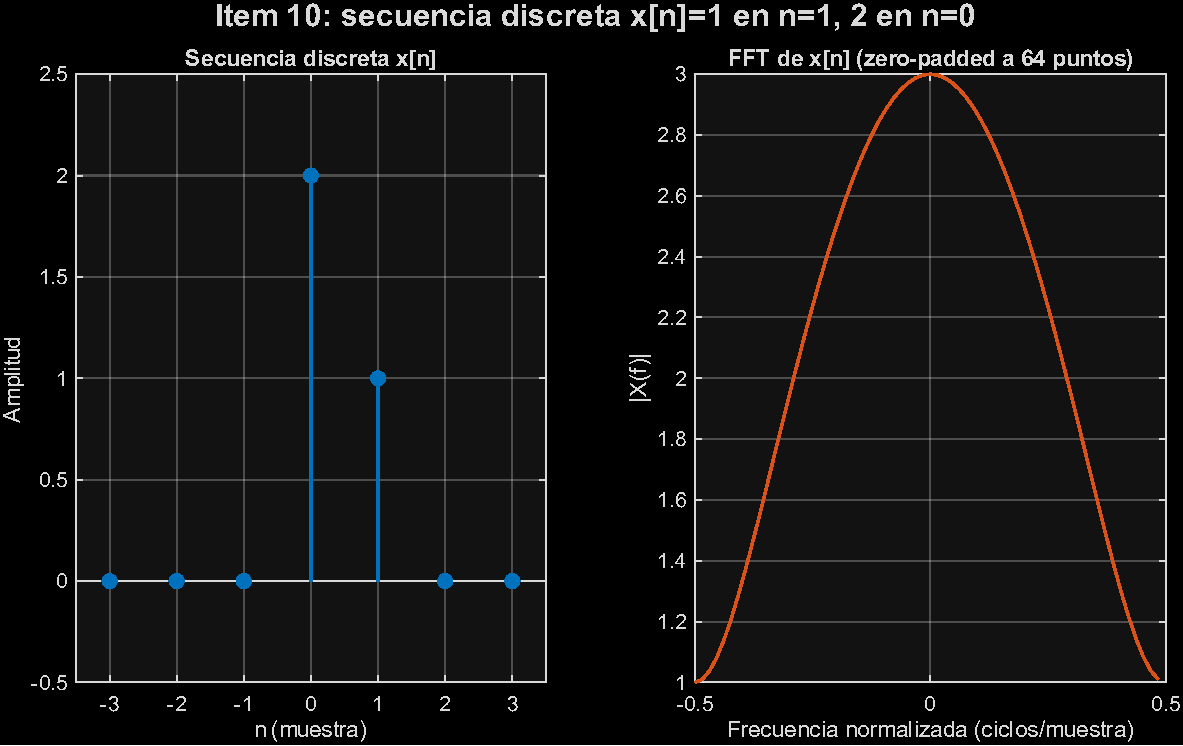
\includegraphics[width=\columnwidth]{images/01_item10_secuencia.pdf}
\caption{Ítem 10: secuencia discreta $x[n]$ ($x[0]{=}2$, $x[1]{=}1$, resto 0), representación \texttt{stem} y FFT con \textit{zero-padding} a 64 puntos.}
\label{fig:item10}
\end{figure}

\subsection{Ítem 11: onda diente de sierra (\textit{sawtooth}), 15~s, $f=1$~Hz}
\textbf{Fase 1.} Como forma de onda ideal es una función matemática, pero su generación física (mediante circuitos de carga/descarga de un capacitor) es común en instrumentación real. \textbf{Fase 2.} La onda diente de sierra es la señal clásica empleada para el barrido temporal en osciloscopios analógicos de rayos catódicos y para la generación de relojes de barrido de frecuencia (\textit{chirp} lineal aproximado) en analizadores de espectro de barrido; su espectro, rico en armónicos de decaimiento $1/k$, la hace poco adecuada como portadora de comunicación pero muy relevante como señal de temporización y sincronización en equipos de prueba. La Figura \ref{fig:item11} muestra la señal sobre los 15~s de duración especificados.

\begin{figure}[!t]
\centering
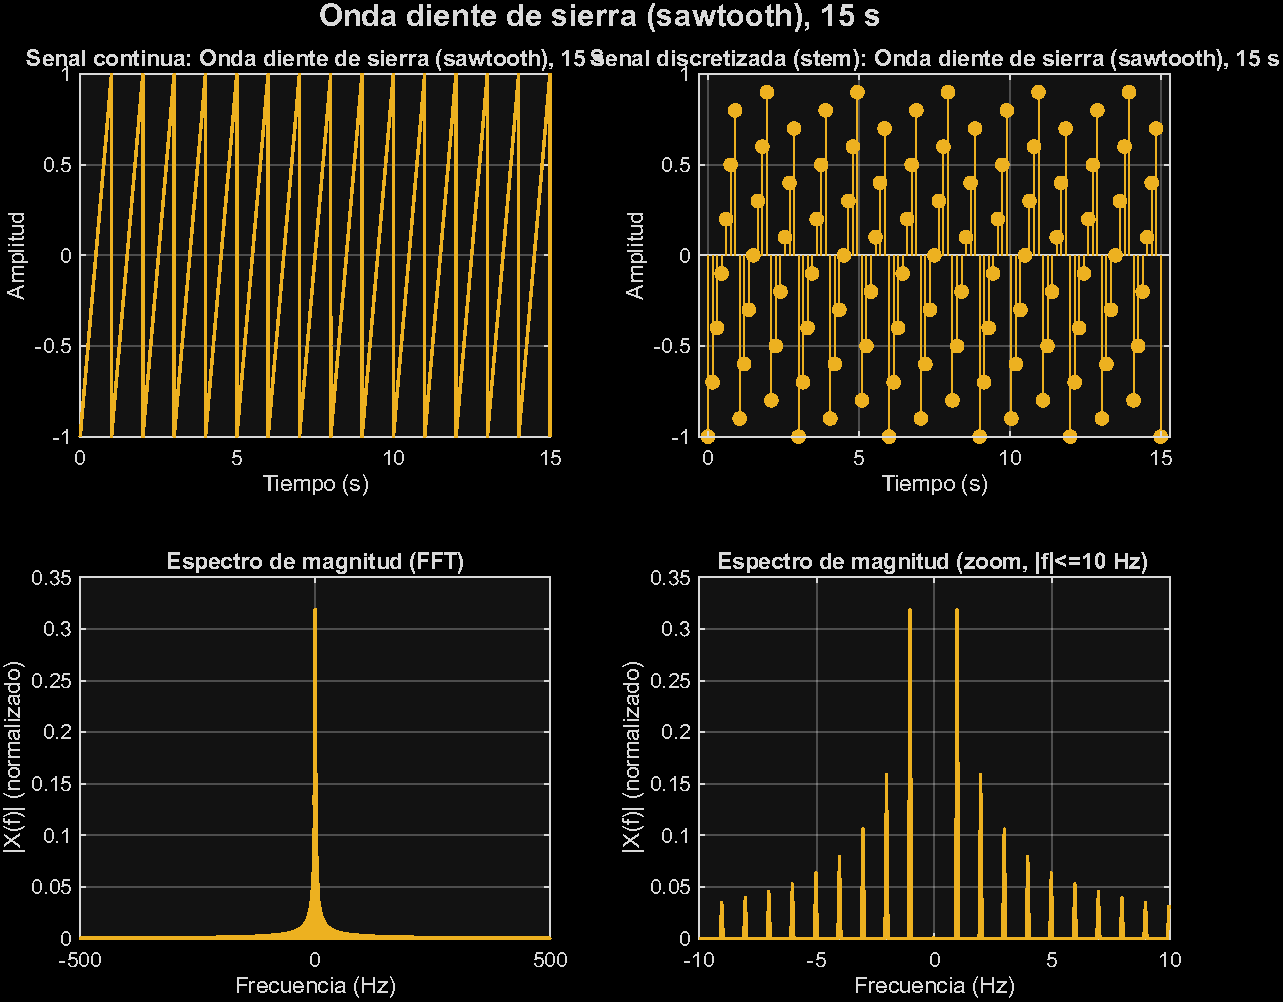
\includegraphics[width=\columnwidth]{images/01_item11_sawtooth.pdf}
\caption{Ítem 11: onda diente de sierra, $f=1$~Hz, duración 15~s, con su discretización y espectro FFT.}
\label{fig:item11}
\end{figure}

\subsection{Ítem 12: $Y_1=A\sin(5\omega t)$, $Y_2=1.2A\sin(4\omega t)$, $Z=Y_1+Y_2$}
\textbf{Fase 1.} Con $A=1$ (supuesto) representa dos señales senoidales de distinta frecuencia y amplitud sumadas; si se interpretan como voltajes, $Z(t)$ representa físicamente la superposición lineal de dos fuentes senoidales sobre una misma carga o conductor. \textbf{Fase 2.} Esta superposición es el modelo directo de la distorsión armónica y de la interferencia entre canales adyacentes: cuando dos señales de frecuencias cercanas pero no armónicamente relacionadas (aquí $4\omega$ y $5\omega$) se suman, el resultado presenta batido (\textit{beating}) y una envolvente moduladora, fenómeno relevante tanto en distorsión de intermodulación de amplificadores no lineales como en la interferencia entre portadoras próximas en un mismo medio de transmisión. La Figura \ref{fig:item12} muestra $Y_1$, $Y_2$ y $Z$ por separado.

\begin{figure}[!t]
\centering
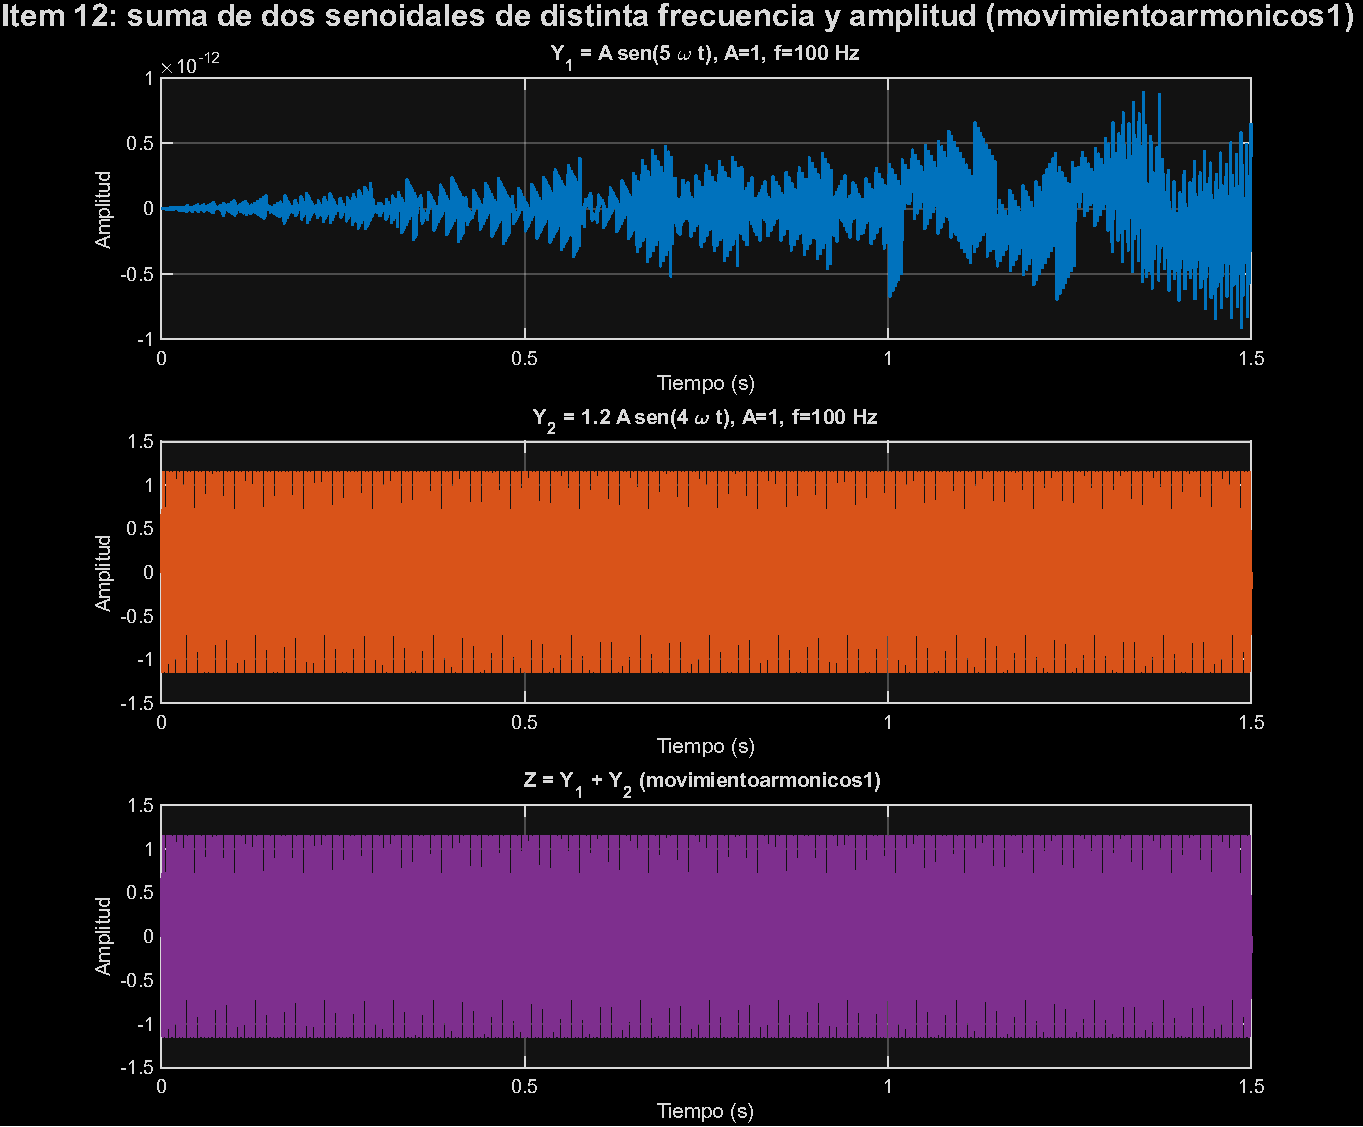
\includegraphics[width=\columnwidth]{images/01_item12_movimientoarmonicos1.pdf}
\caption{Ítem 12: $Y_1=A\sin(5\omega t)$, $Y_2=1.2A\sin(4\omega t)$ y $Z=Y_1+Y_2$, con $\omega=2\pi(100)$ rad/s y $A=1$ (supuesto).}
\label{fig:item12}
\end{figure}

\subsection{Ítems 1, 3, 4 y 8: figuras complementarias}

Por razones de espacio, las señales de los ítems 1, 3, 4 y 8, ya interpretadas anteriormente, se agrupan en la Figura \ref{fig:grid1} en formato reducido, junto con sus espectros de magnitud correspondientes.

\begin{figure}[!t]
\centering
\begin{minipage}{0.49\columnwidth}
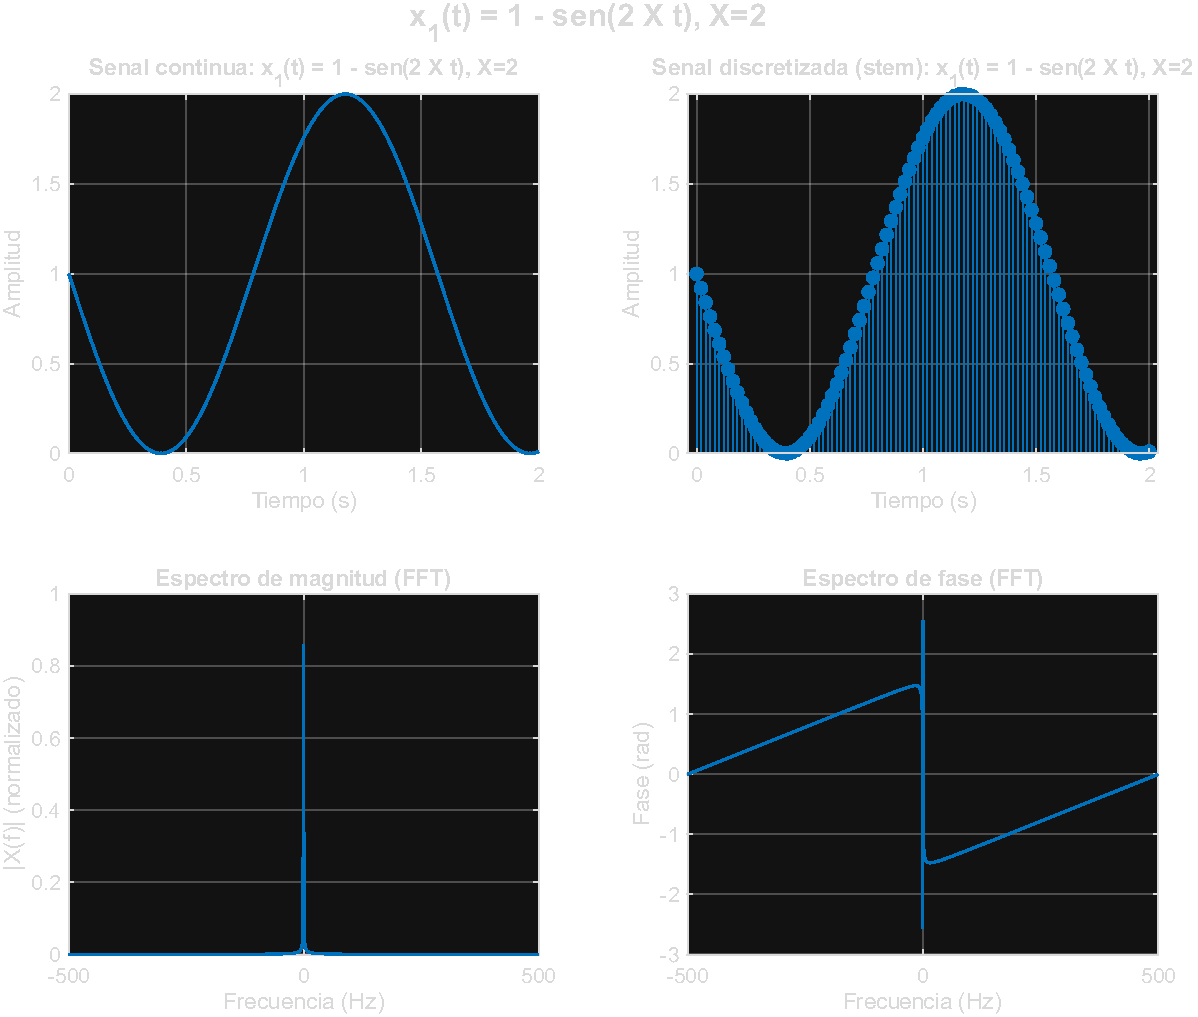
\includegraphics[width=\linewidth]{images/01_item01_uno_menos_sen.pdf}
\end{minipage}\hfill
\begin{minipage}{0.49\columnwidth}
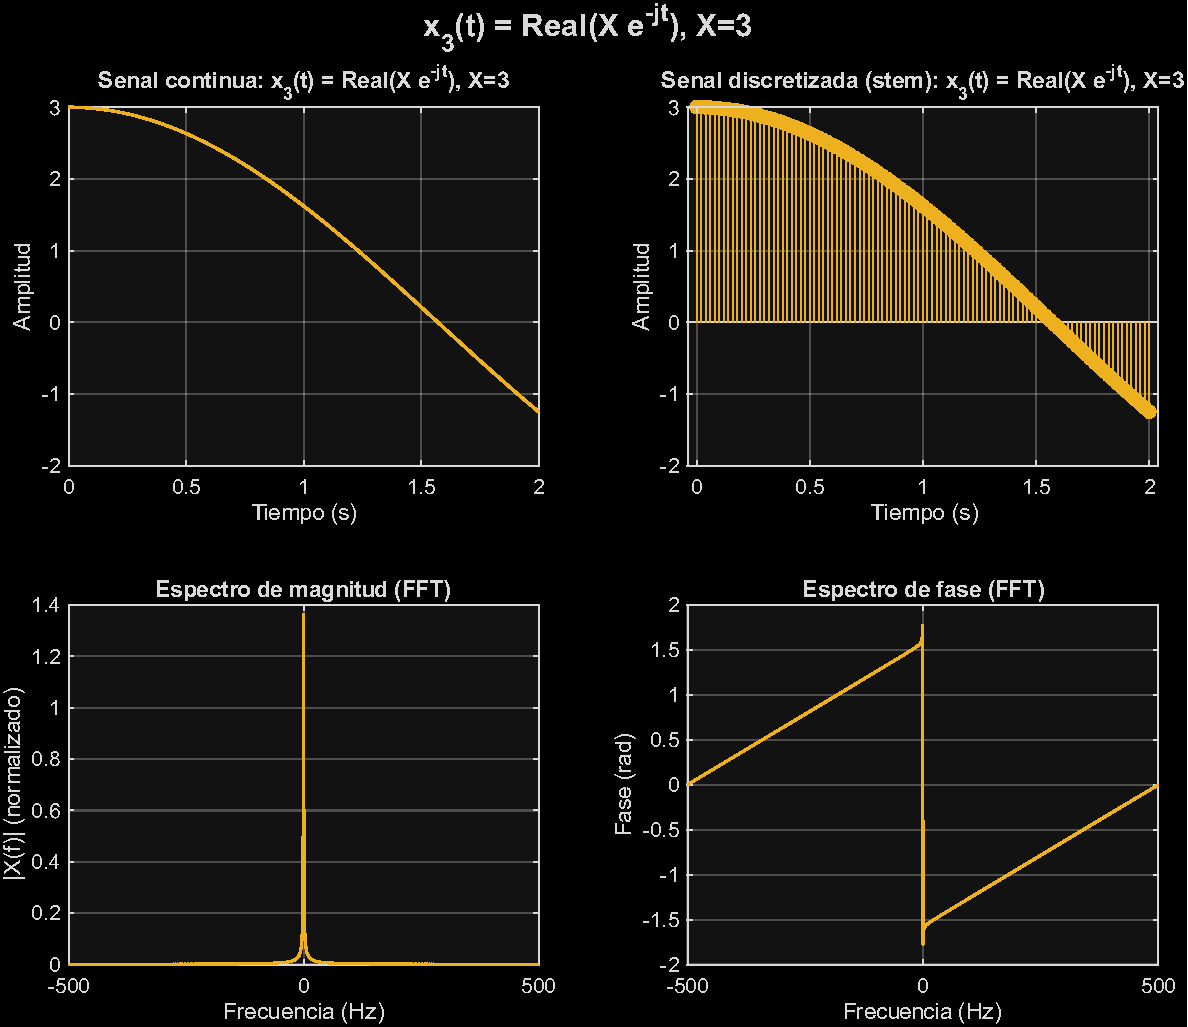
\includegraphics[width=\linewidth]{images/01_item03_real_exp.pdf}
\end{minipage}

\vspace{0.3em}
\begin{minipage}{0.49\columnwidth}
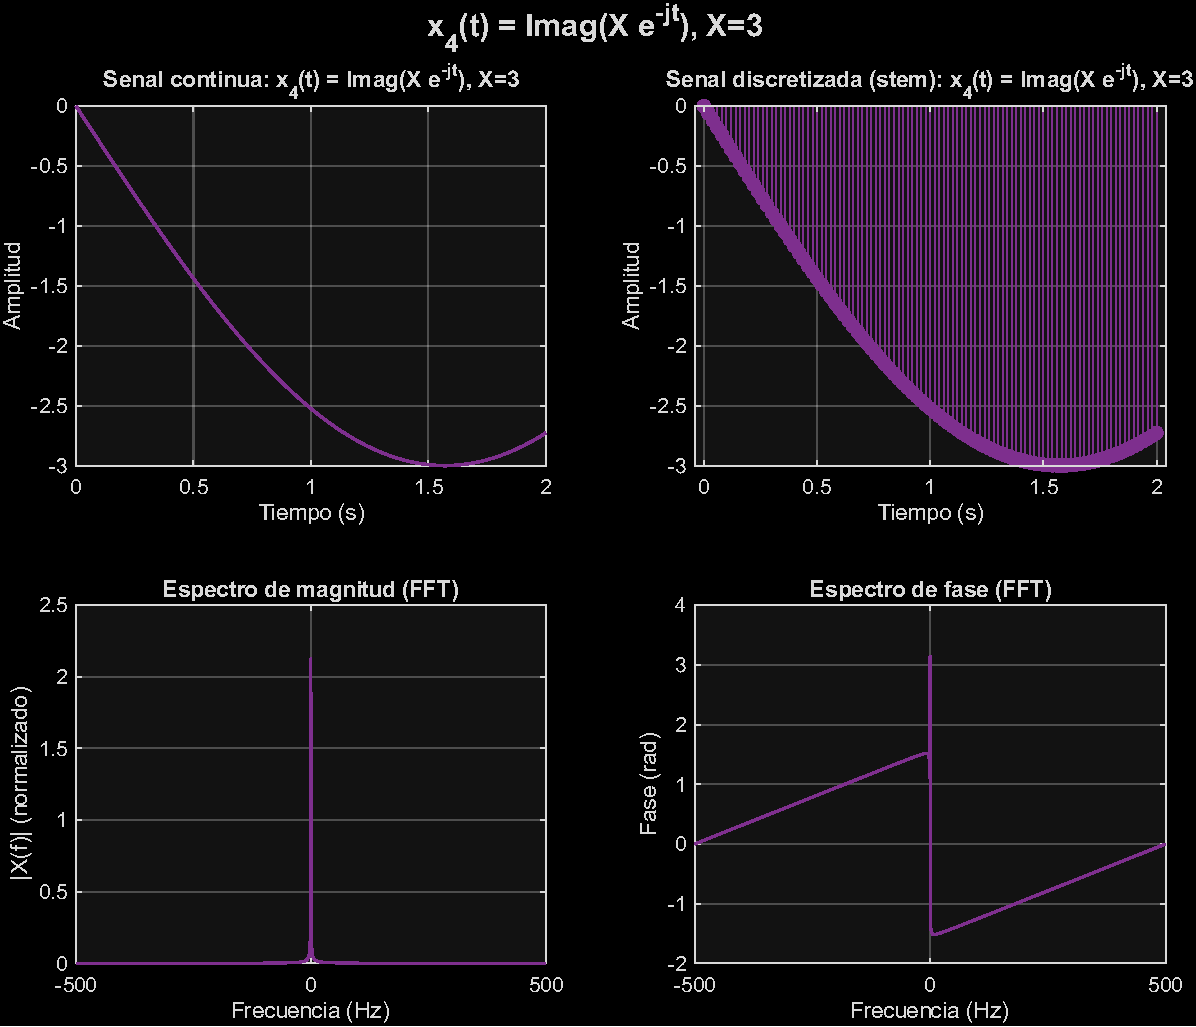
\includegraphics[width=\linewidth]{images/01_item04_imag_exp.pdf}
\end{minipage}\hfill
\begin{minipage}{0.49\columnwidth}
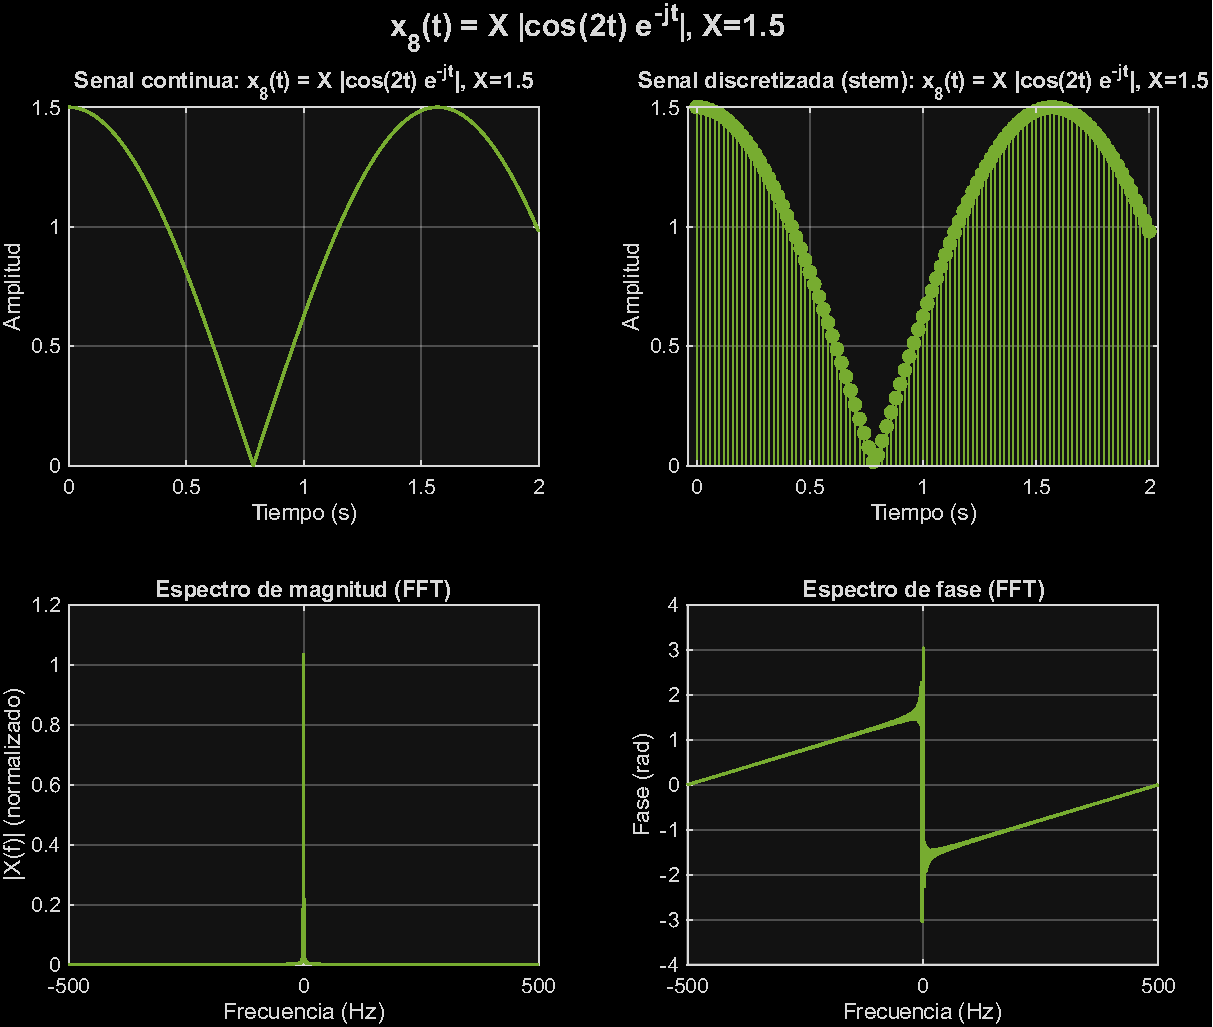
\includegraphics[width=\linewidth]{images/01_item08_abs_cos_exp.pdf}
\end{minipage}
\caption{Señales complementarias: ítem 1 ($1-\sin(2Xt)$, arriba izq.), ítem 3 ($\text{Re}\{Xe^{-jt}\}=3\cos(t)$, arriba der.), ítem 4 ($\text{Im}\{Xe^{-jt}\}=-3\sin(t)$, abajo izq.) e ítem 8 ($1.5|\cos(2t)e^{-jt}|$, abajo der.).}
\label{fig:grid1}
\end{figure}

\subsection{Señal senoidal amortiguada}

Como complemento del ejercicio, se simuló la señal $X(t)=e^{-0.1t}\sin(0.6666t)$ sobre $t=0$:$0.1$:$30$~s, graficada hasta $t=35$~s con amplitud limitada a $[-1,1]$ (Figura \ref{fig:amortiguada}). \textbf{Fase 1 (modelado).} Representa el comportamiento típico de un sistema físico de segundo orden subamortiguado, por ejemplo, la respuesta transitoria de corriente o voltaje en un circuito RLC subamortiguado, o la respuesta mecánica de un sistema masa-resorte-amortiguador; la envolvente exponencial decae a $e^{-3}\approx0.0498$ hacia $t=30$~s, por lo que la amplitud es prácticamente nula al final del intervalo graficado. \textbf{Fase 2 (interpretación técnica).} En telecomunicaciones, una respuesta de este tipo es característica de la respuesta al escalón de un filtro o de una línea de transmisión con reflexión parcial (desadaptación de impedancia), donde la energía reflejada decae con el tiempo debido a las pérdidas del medio; también modela el tiempo de establecimiento (\textit{settling time}) de un oscilador o un lazo de enganche de fase (PLL) tras una perturbación, magnitud crítica para determinar cuánto debe esperar un receptor antes de considerar estable una señal recuperada.

\begin{figure}[!t]
\centering
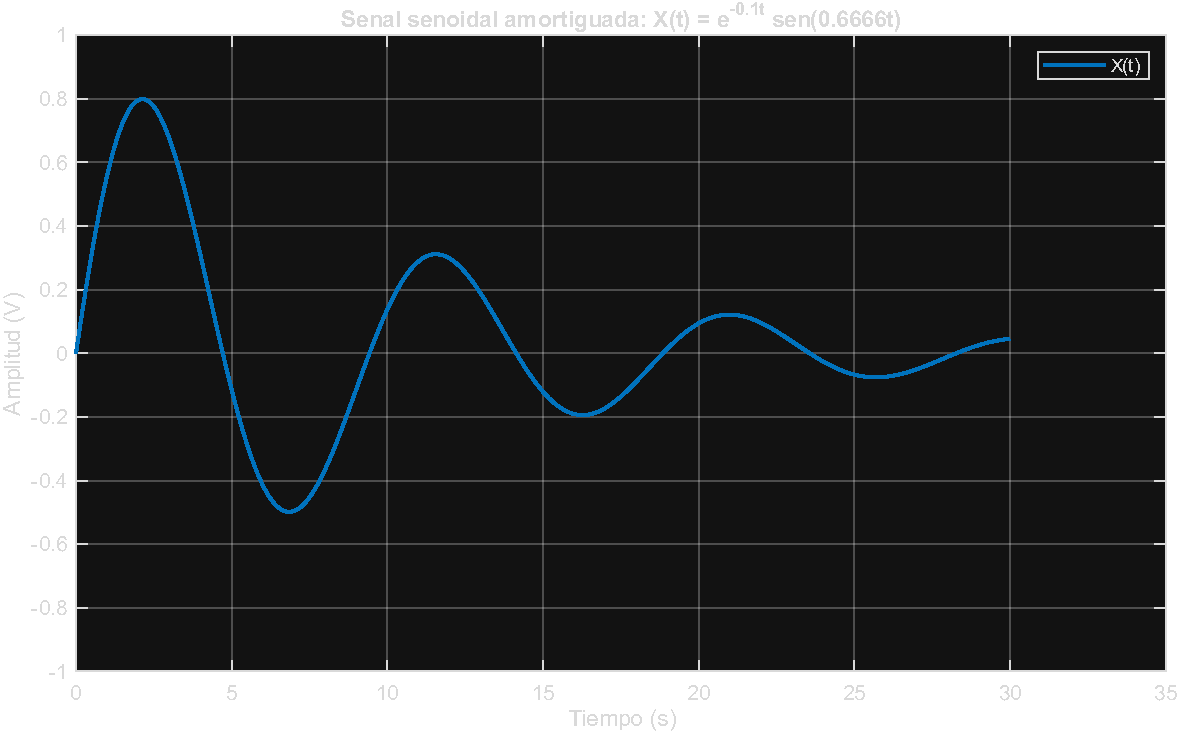
\includegraphics[width=\columnwidth]{images/02_senal_amortiguada.pdf}
\caption{Señal senoidal amortiguada $X(t)=e^{-0.1t}\sin(0.6666t)$, $t=0$ a 30~s (graficada hasta 35~s), ejes fijados a $[-1,1]$.}
\label{fig:amortiguada}
\end{figure}

\subsection{Síntesis del Ejercicio 1}

La Tabla \ref{tab:resumen_ej1} sintetiza, para cada uno de los doce ítems, si la señal corresponde a una cantidad física realizable o a una función matemática abstracta, y su principal aplicación análoga en telecomunicaciones.

\begin{table}[!t]
\centering
\caption{Síntesis de interpretación física y técnica de las señales del Ejercicio 1}
\label{tab:resumen_ej1}
\begin{tabular}{|c|l|l|}
\hline
\textbf{Ítem} & \textbf{Naturaleza} & \textbf{Aplicación análoga} \\ \hline
1 & Abstracta & Offset de polarización \\ \hline
2 & Abstracta & Muestreo/reconstrucción ideal \\ \hline
3 & Física/circuital & Fasor de CA, banda base I \\ \hline
4 & Física/circuital & Banda base Q (cuadratura) \\ \hline
5 & Idealización & Transitorio de conmutación \\ \hline
6 & Física (voltaje) & Señalización digital NRZ \\ \hline
7 & Abstracta & Inestabilidad/realimentación \\ \hline
8 & Abstracta & Rectificación de onda completa \\ \hline
9 & Abstracta & Filtro pasa-bajas ideal \\ \hline
10 & Abstracta (discreta) & Símbolos/filtro FIR digital \\ \hline
11 & Física (osciloscopio) & Barrido de frecuencia/reloj \\ \hline
12 & Física (voltaje) & Distorsión/interferencia \\ \hline
\end{tabular}
\end{table}

\section{Resultados: Ejercicio 3 (Armónicos de 60~Hz)}

\subsection{Fase 1: Modelado}

Se generaron los seis armónicos individuales $y_k(t) = A_k\sin(2\pi k f t)$, $k=1,\dots,6$, con $f=60$~Hz y amplitudes $A_k = [120,60,40,30,24,20]$~V, mostrados por separado en la Figura \ref{fig:armonicos_ind} y superpuestos en un mismo eje en la Figura \ref{fig:armonicos_sup}. La señal resultante $y_{sum}(t)=\sum_{k=1}^{6}y_k(t)$ se muestra en la Figura \ref{fig:senal_suma}: su forma ya no es una senoidal pura, sino que presenta picos y valles adicionales característicos de la distorsión armónica producida por cargas no lineales.

\begin{figure}[!t]
\centering
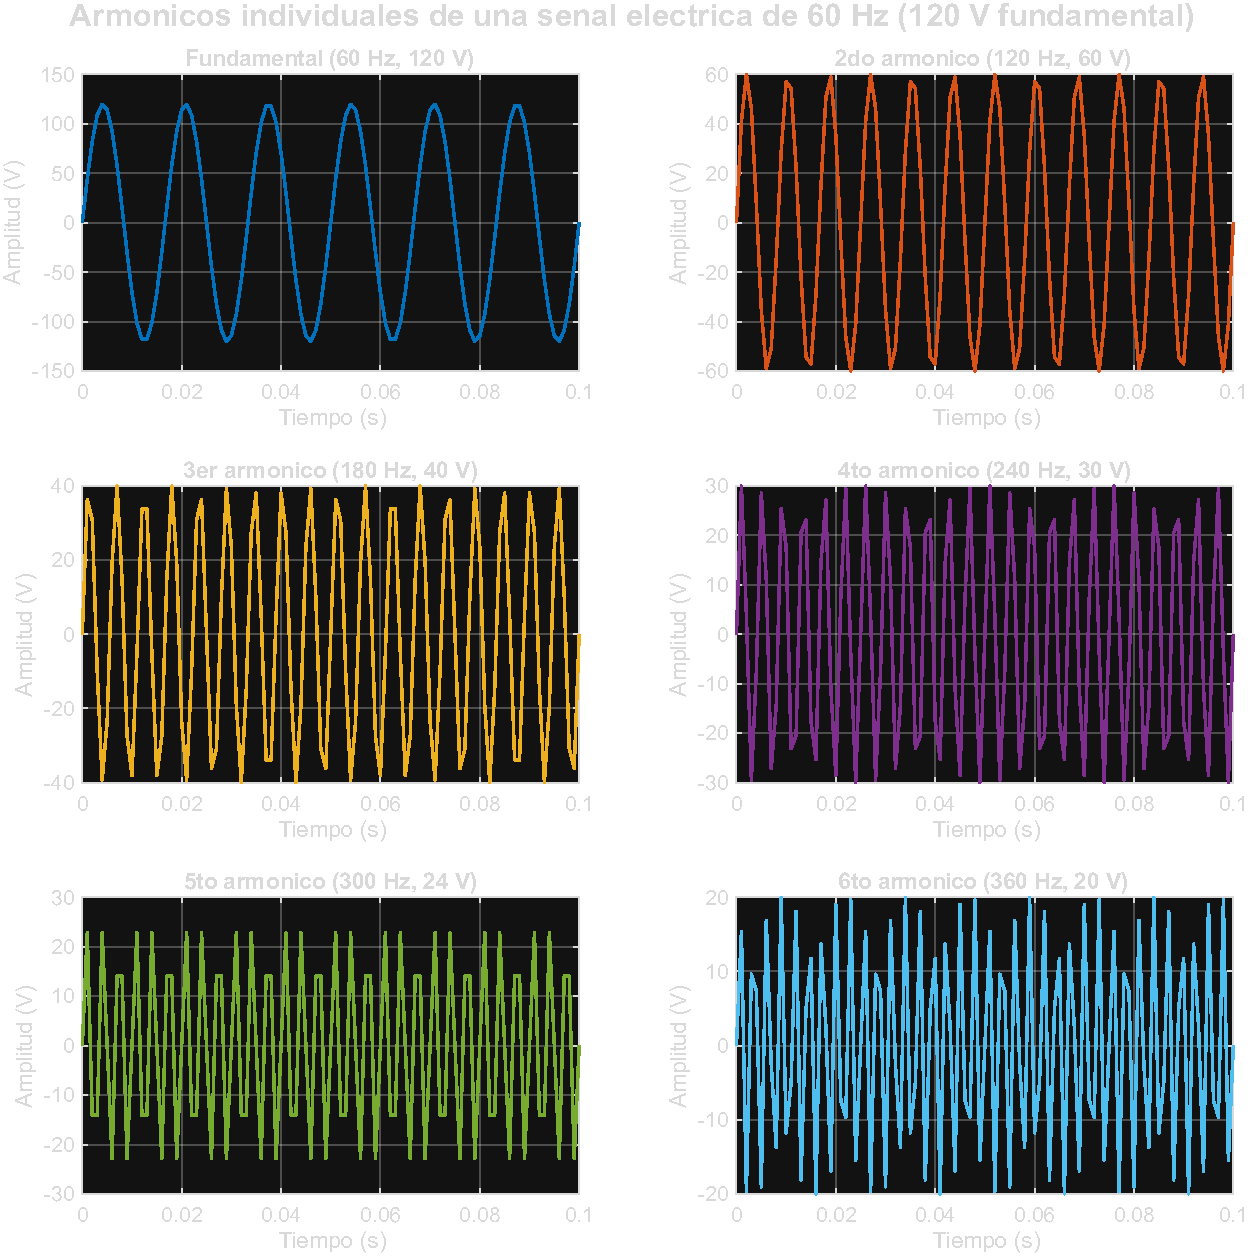
\includegraphics[width=\columnwidth]{images/03a_armonicos_individuales.pdf}
\caption{Seis armónicos individuales de una señal eléctrica de 60~Hz (fundamental 120~V hasta el 6.\textsuperscript{o} armónico, 20~V), ventana de 6 ciclos de la fundamental (0 a 0.1~s).}
\label{fig:armonicos_ind}
\end{figure}

\begin{figure}[!t]
\centering
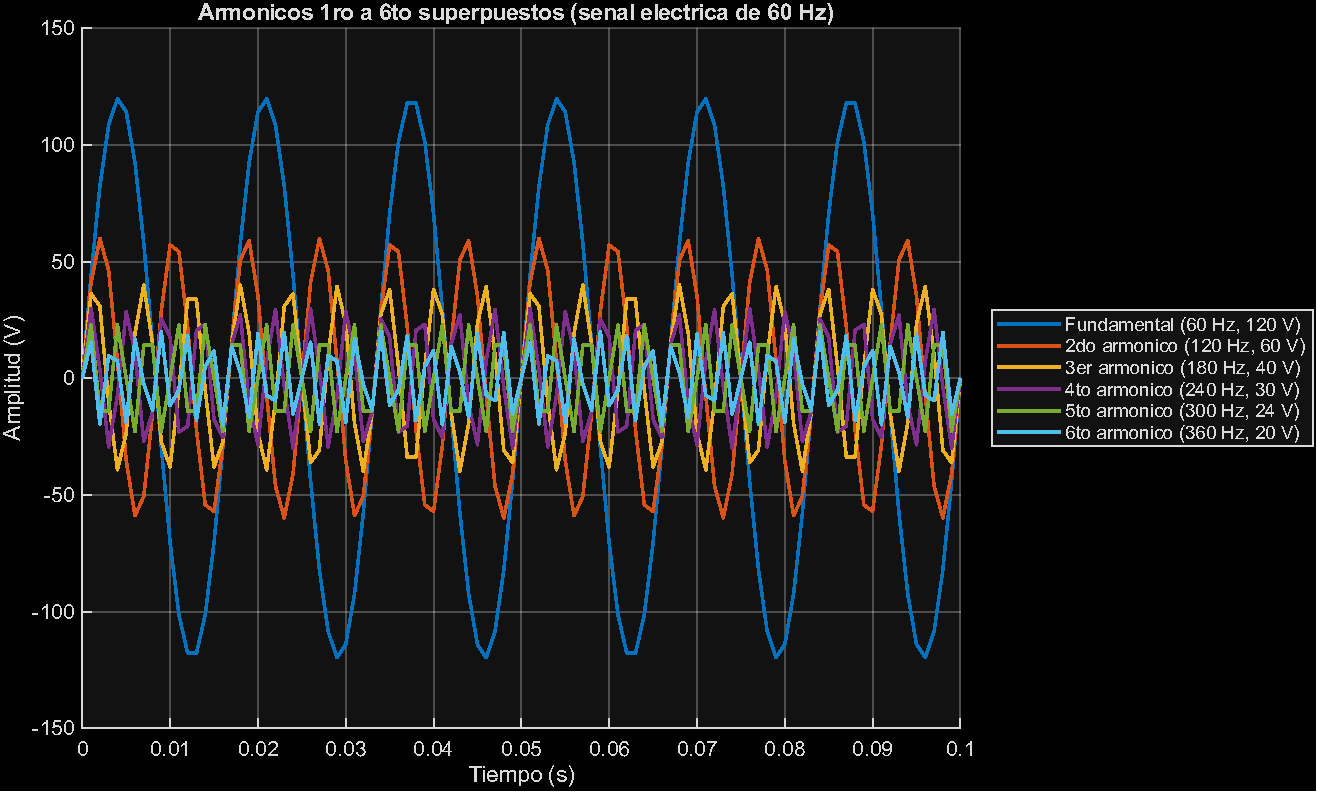
\includegraphics[width=\columnwidth]{images/03b_armonicos_superpuestos.pdf}
\caption{Los seis armónicos superpuestos en un mismo eje, permitiendo comparar sus amplitudes y frecuencias relativas.}
\label{fig:armonicos_sup}
\end{figure}

\begin{figure}[!t]
\centering
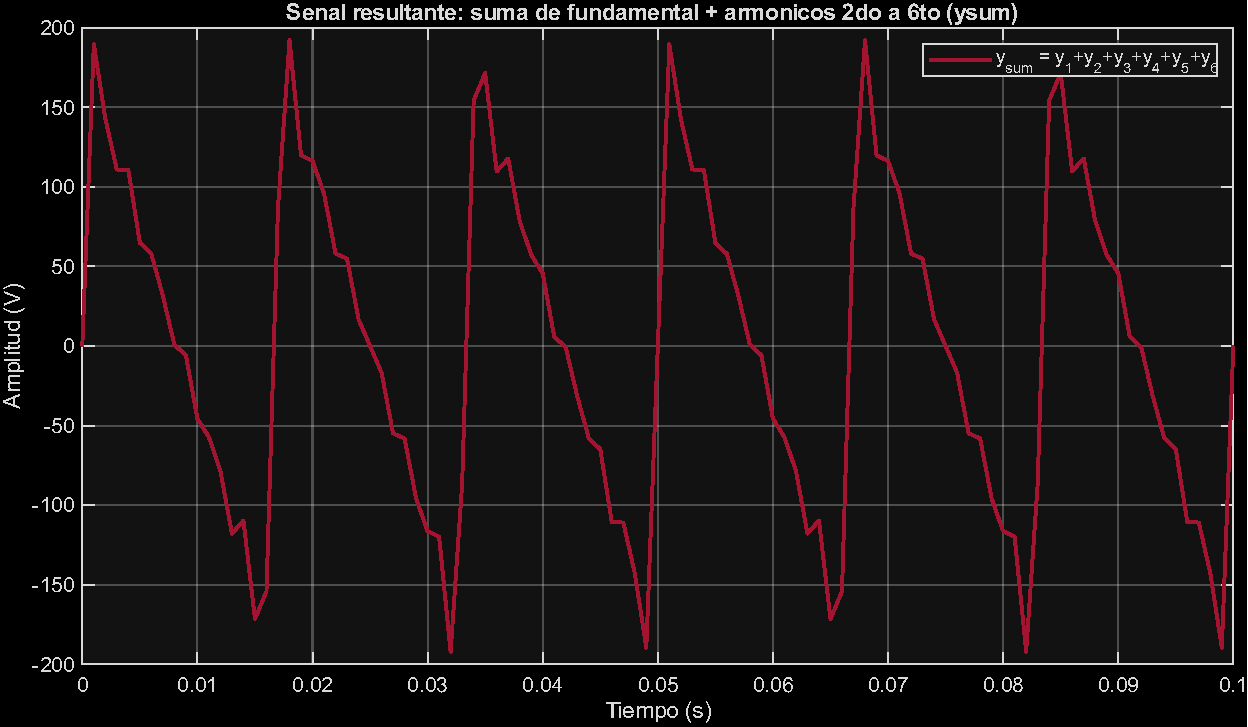
\includegraphics[width=\columnwidth]{images/03c_senal_suma.pdf}
\caption{Señal resultante $y_{sum}$ (fundamental más cinco armónicos), mostrando la distorsión típica de cargas no lineales.}
\label{fig:senal_suma}
\end{figure}

\subsection{Fase 2: Análisis de frecuencia y efecto de parámetros}

\textbf{¿Cuál es la frecuencia dominante de la señal resultante?} La componente dominante en amplitud sigue siendo la fundamental de 60~Hz (120~V), pues su amplitud es mayor que la de cualquier armónico individual; sin embargo, la forma de onda temporal ya no es puramente senoidal a 60~Hz, sino la superposición de las seis componentes, por lo que la ``frecuencia dominante'' en sentido espectral (60~Hz) no coincide con la frecuencia de repetición aparente de picos y valles de la forma de onda deformada, que refleja la interacción de todas las componentes armónicas.

\textbf{¿Qué ocurre si cambia el amortiguamiento?} Es importante notar que la señal de este ejercicio (suma de armónicos de 60~Hz) no incluye ningún término de amortiguamiento exponencial: cada componente $y_k(t)$ es una senoidal de amplitud constante en el tiempo, a diferencia de la señal amortiguada $X(t)=e^{-0.1t}\sin(0.6666t)$ analizada en la Sección V (Señal senoidal amortiguada). Esta pregunta, procedente de una plantilla de guía reutilizada entre ejercicios del laboratorio, se interpreta aquí en su sentido genérico aplicable a sistemas de segundo orden: de existir amortiguamiento (por ejemplo, si la señal representase la respuesta transitoria de un transformador o inductor ante un evento de conmutación superpuesto a la componente armónica en estado estacionario), un mayor coeficiente de amortiguamiento reduciría más rápidamente la amplitud de las componentes transitorias, dejando únicamente el contenido armónico en estado estacionario aquí analizado; un menor amortiguamiento prolongaría la coexistencia de transitorios y armónicos, complicando su separación espectral.

\textbf{¿Qué ocurre si aumenta la frecuencia fundamental?} Si la frecuencia fundamental $f$ aumentara (por ejemplo, en un sistema de 50~Hz que migrara a 60~Hz, o en presencia de variaciones de frecuencia de red), todos los armónicos se desplazarían proporcionalmente ($k\cdot f$ para cada orden $k$), separándose más entre sí en el dominio de la frecuencia (mayor separación absoluta en Hz entre armónicos consecutivos) pero manteniendo la misma proporción relativa; con la resolución espectral fija de la FFT empleada ($\Delta f\approx9.99$~Hz), un aumento de $f$ facilitaría ligeramente la discriminación de picos vecinos, mientras que una disminución de $f$ los acercaría, exigiendo mayor duración de ventana para mantener la misma resolución relativa según la ecuación \eqref{eq:resolucion}.

\subsection{Fase 3: Interpretación técnica}

El espectro de magnitud de $y_{sum}$, mostrado en la Figura \ref{fig:espectro_ysum}, confirma la composición armónica esperada mediante picos en 60, 120, 180, 240, 300 y 360~Hz. Aplicando la ecuación \eqref{eq:thd} con las amplitudes de diseño:
\begin{equation}
\text{THD} = \frac{\sqrt{60^2+40^2+30^2+24^2+20^2}}{120} \approx \frac{84.12}{120} \approx 70.1\%
\label{eq:thd_calculo}
\end{equation}
un valor de THD extremadamente alto para un sistema eléctrico real (las normas como IEEE 519 típicamente exigen THD inferior al 5--8\% en el punto de acoplamiento común), y notablemente influenciado por el segundo armónico, que por sí solo representa el 50\% de la amplitud de la fundamental. En un sistema eléctrico real, un THD de esta magnitud provocaría sobrecalentamiento apreciable de conductores y transformadores por pérdidas adicionales de efecto piel y corrientes de Foucault, interferencia electromagnética significativa hacia equipos de comunicación y control cercanos a la instalación, y errores relevantes en instrumentos de medición que asumen una onda senoidal pura, motivando en la práctica el uso de filtros de armónicos y transformadores con capacidad de derrateo (\textit{K-factor}) diseñados específicamente para operar bajo cargas no lineales.

\begin{figure}[!t]
\centering
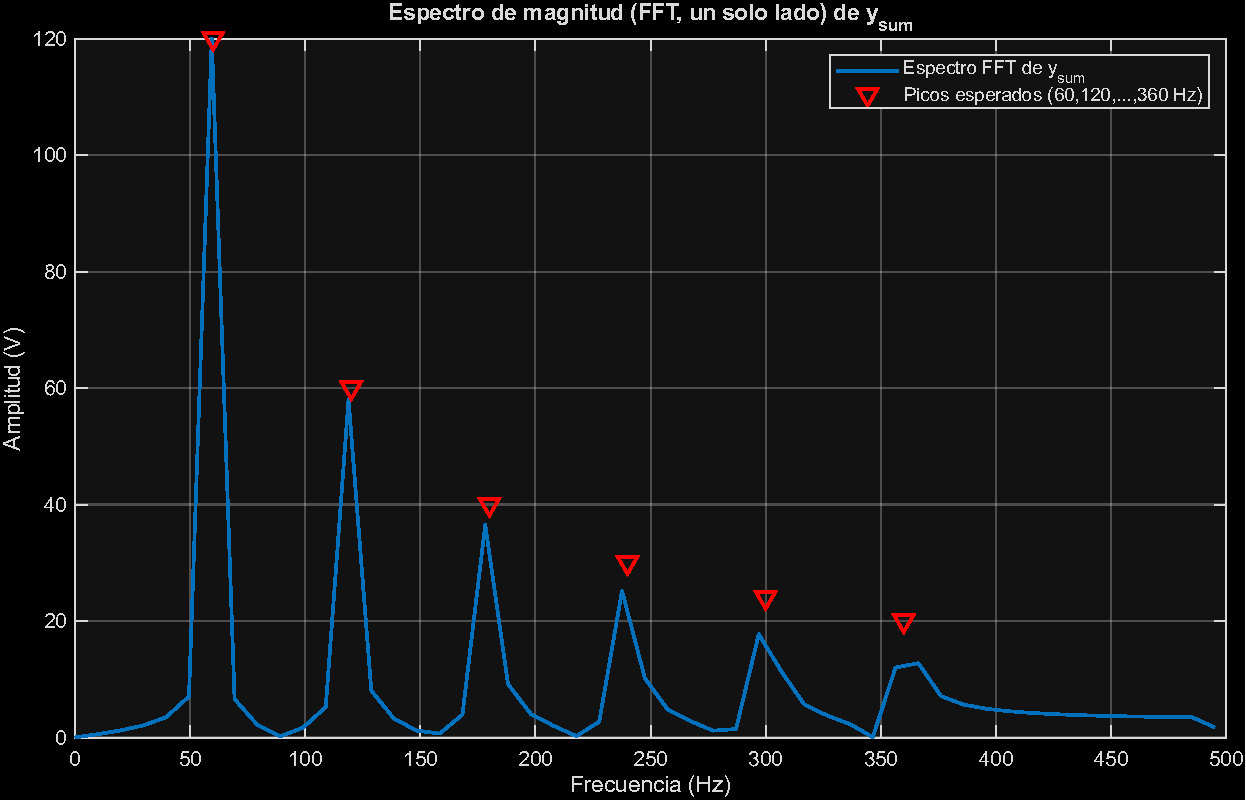
\includegraphics[width=\columnwidth]{images/03d_espectro_ysum.pdf}
\caption{Espectro de magnitud (FFT, un solo lado) de $y_{sum}$, con picos esperados en 60, 120, 180, 240, 300 y 360~Hz (triángulos rojos) y amplitudes decrecientes 120, 60, 40, 30, 24 y 20~V. $F_s=1000$~Hz, $N=101$ muestras, $\Delta f\approx9.9$~Hz.}
\label{fig:espectro_ysum}
\end{figure}

\subsection{Fase 4: Modelo Simulink y validación experimental}

La Figura \ref{fig:simulink_diagrama} muestra la arquitectura de bloques del modelo \texttt{modelo\_armonicos\_60hz}: seis bloques \textit{Sine Wave} (uno por armónico) alimentan un bloque \textit{Add} de seis entradas (\texttt{Suma\_armonicos}), cuya salida se bifurca hacia un bloque \textit{Scope} (dominio del tiempo), un bloque \textit{Spectrum Analyzer} (dominio de la frecuencia, condicionado a la \textit{DSP System Toolbox}) y un bloque \textit{To Workspace} que exporta la señal muestreada para análisis posterior en MATLAB. La Figura \ref{fig:simulink_tiempo} muestra la forma de onda temporal resultante, obtenida desde la variable exportada, y la Figura \ref{fig:simulink_fft} su espectro FFT.

\begin{figure}[!t]
\centering
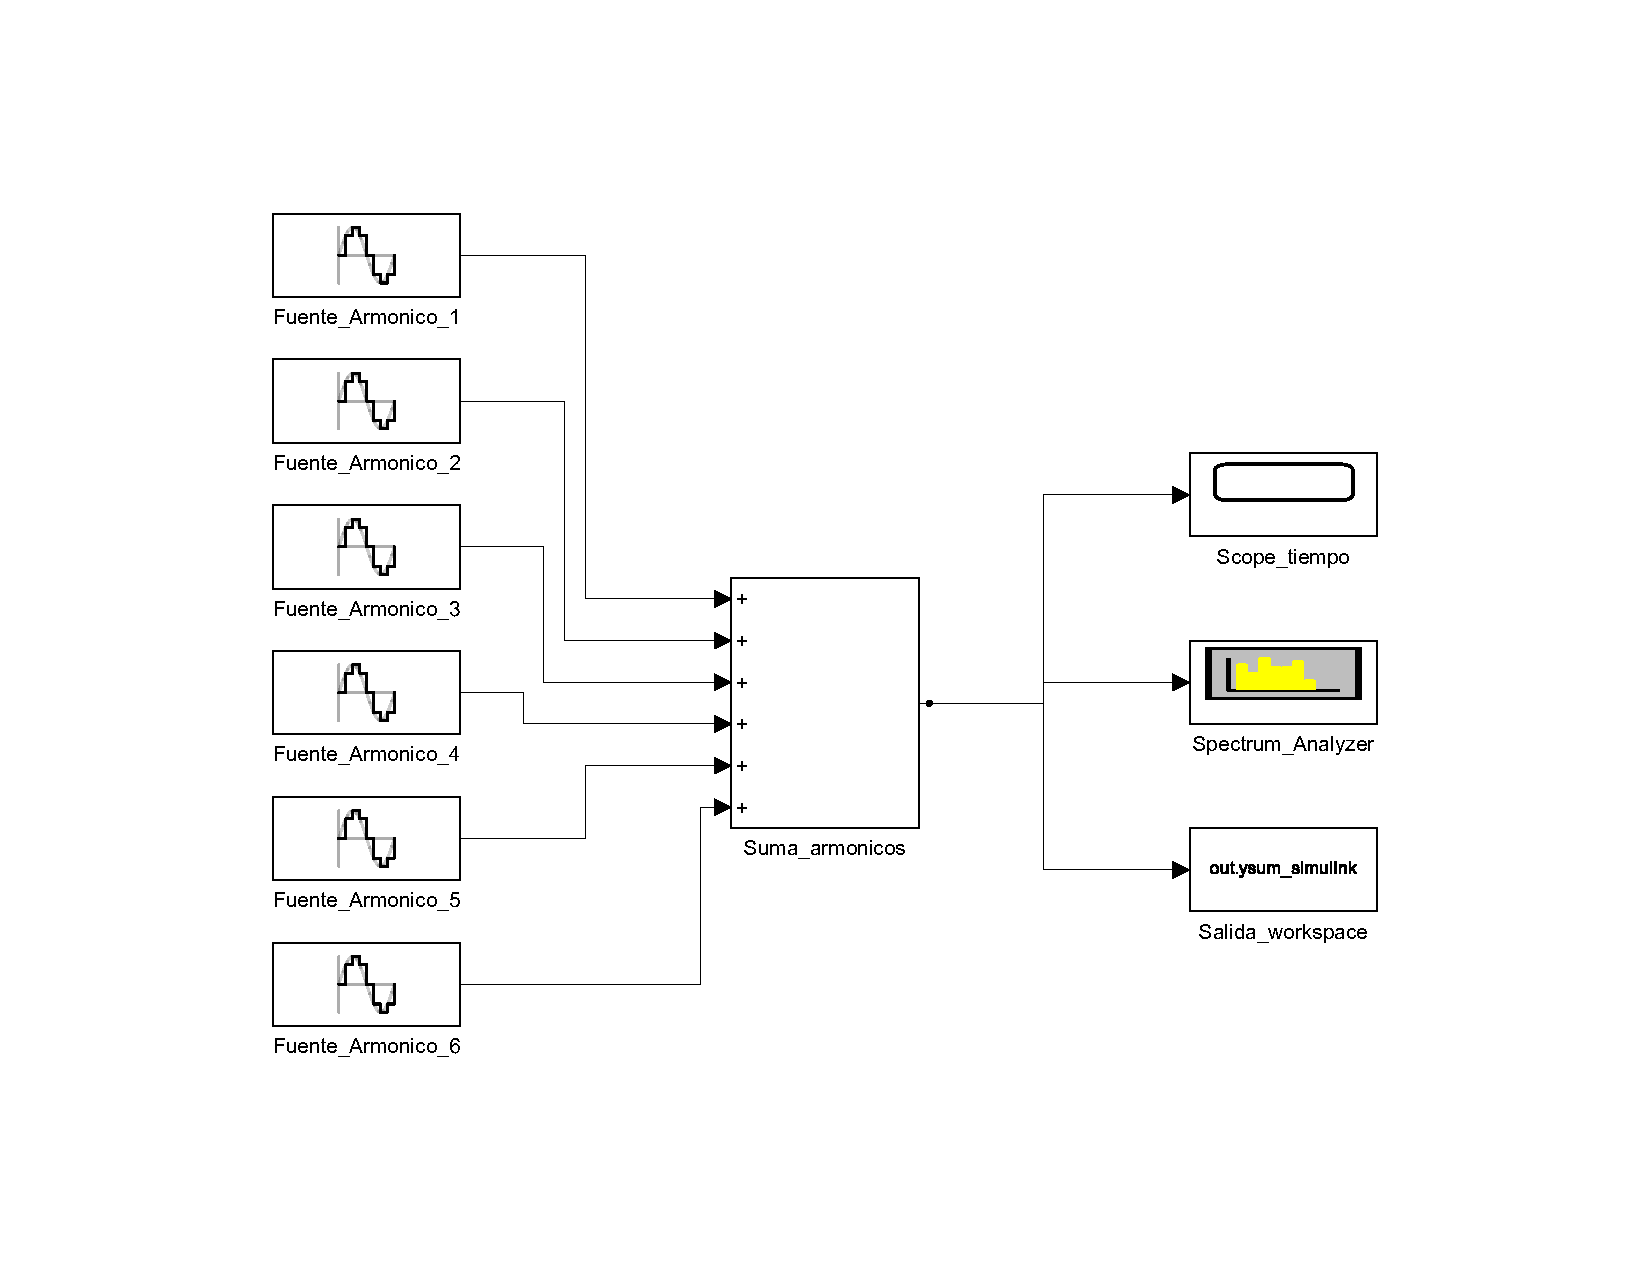
\includegraphics[width=\columnwidth]{images/04c_simulink_diagrama.pdf}
\caption{Diagrama de bloques del modelo Simulink \texttt{modelo\_armonicos\_60hz}: seis fuentes \textit{Sine Wave} $\rightarrow$ \textit{Add} (\texttt{Suma\_armonicos}) $\rightarrow$ \textit{Scope}, \textit{Spectrum Analyzer} y \textit{To Workspace}.}
\label{fig:simulink_diagrama}
\end{figure}

\begin{figure}[!t]
\centering
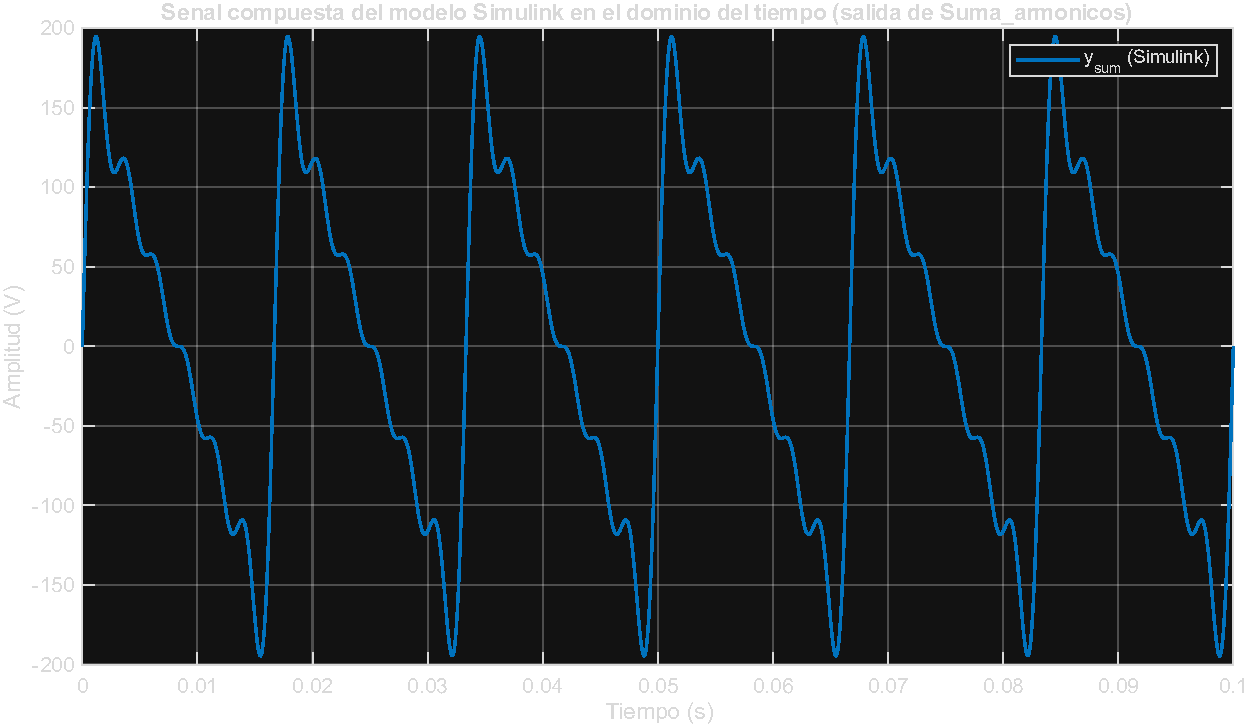
\includegraphics[width=\columnwidth]{images/04a_simulink_tiempo.pdf}
\caption{Forma de onda en el dominio del tiempo de la señal compuesta simulada en Simulink (equivalente a lo que mostraría el bloque \textit{Scope}), $F_s=10\,000$~Hz, duración 0.1~s.}
\label{fig:simulink_tiempo}
\end{figure}

\begin{figure}[!t]
\centering
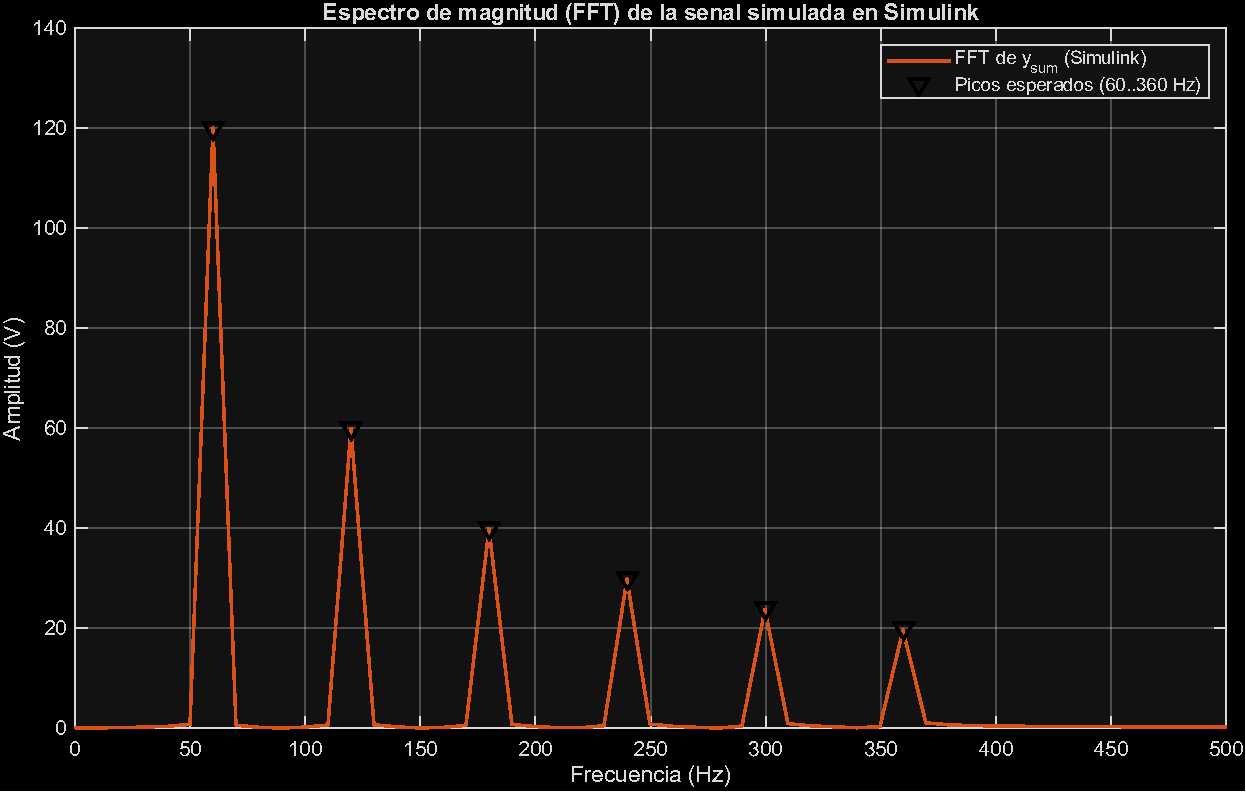
\includegraphics[width=\columnwidth]{images/04b_simulink_fft.pdf}
\caption{Espectro de magnitud (FFT, un solo lado) de la señal registrada desde Simulink vía \textit{To Workspace}, con picos esperados marcados en 60, 120, 180, 240, 300 y 360~Hz (triángulos negros). $F_s=10\,000$~Hz, $N=1001$ muestras, $\Delta f=9.990$~Hz.}
\label{fig:simulink_fft}
\end{figure}

La Tabla \ref{tab:simulink_valores} compara los valores de diseño con los picos detectados automáticamente mediante \texttt{findpeaks} sobre el espectro exportado desde Simulink.

\begin{table}[!t]
\centering
\caption{Comparación entre valores de diseño y picos detectados en la FFT de Simulink}
\label{tab:simulink_valores}
\begin{tabular}{|c|c|c|c|c|}
\hline
\textbf{Arm.} & \textbf{$f$ diseño (Hz)} & \textbf{$f$ detect. (Hz)} & \textbf{$A$ diseño (V)} & \textbf{$A$ detect. (V)} \\ \hline
1 & 60.0 & 59.940 & 120.0 & 120.075 \\ \hline
2 & 120.0 & 119.880 & 60.0 & 59.969 \\ \hline
3 & 180.0 & 179.820 & 40.0 & 39.898 \\ \hline
4 & 240.0 & 239.760 & 30.0 & 29.828 \\ \hline
5 & 300.0 & 299.700 & 24.0 & 23.744 \\ \hline
6 & 360.0 & 359.640 & 20.0 & 19.604 \\ \hline
\end{tabular}
\end{table}

Los seis picos detectados caen dentro de 0.06~Hz de las frecuencias de diseño (una fracción menor de la resolución espectral $\Delta f = 9.99$~Hz) y las amplitudes detectadas coinciden con las de diseño con un error inferior al 2\% en todos los casos. Con $F_s=10\,000$~Hz (muy por encima de $2\times360$~Hz, el requisito de Nyquist para el armónico más alto) y una ventana de 0.1~s que contiene exactamente 6 periodos completos de la fundamental de 60~Hz, esta configuración particular evita tanto el aliasing como la fuga espectral significativa.

\textbf{¿Por qué está mal el espectro? ¿Qué parámetro debe corregirse?} En esta corrida concreta, el espectro obtenido \emph{no está mal}: coincide con los valores de diseño dentro del margen esperable de la resolución finita de la FFT, como se documenta en la Tabla \ref{tab:simulink_valores}. La pregunta del enunciado, sin embargo, es una pregunta de plantilla genérica que interesa responder conceptualmente, pues resulta aplicable a otras configuraciones de parámetros donde el espectro sí podría degradarse. Las cuatro causas típicas por las que un espectro simulado podría resultar incorrecto, y su corrección asociada, son:
\begin{enumerate}
    \item \textbf{Aliasing por muestreo insuficiente:} si $F_s$ no satisface Nyquist ($F_s < 2f_{max}$) para el armónico de mayor orden, dicho armónico se replegaría hacia una frecuencia falsa dentro de la banda base. Corrección: aumentar $F_s$ del solver con margen suficiente (idealmente $F_s \geq 10 f_{max}$).
    \item \textbf{Fuga espectral (\textit{leakage}) por ventana no entera en periodos:} si la duración de la ventana analizada no contiene un número entero de periodos de la fundamental, la FFT asume periodicidad artificial en los bordes y dispersa la energía de cada armónico hacia \textit{bins} vecinos. Corrección: ajustar el tiempo de simulación a un múltiplo entero del periodo fundamental, o aplicar una ventana de suavizado (Hann, Hamming) antes de la FFT.
    \item \textbf{Resolución en frecuencia insuficiente:} si $N$ es demasiado pequeño, $\Delta f = F_s/N$ puede superar la separación entre armónicos (60~Hz), causando que picos cercanos se mezclen. Corrección: aumentar $N$ (mayor tiempo de simulación o menor $T_s$).
    \item \textbf{Configuración del bloque \textit{Spectrum Analyzer}/FFT:} parámetros por defecto (tamaño de FFT, tipo de ventana, promediado, escala lineal vs. dB) pueden dar la impresión de un espectro incorrecto cuando en realidad solo está escalado o ventaneado de forma distinta a la esperada. Corrección: revisar y ajustar explícitamente estos parámetros en el bloque.
\end{enumerate}
En síntesis, en configuraciones donde el espectro sí resultase incorrecto, el parámetro más probable a corregir sería el tiempo de muestreo ($T_s$/$F_s$) para garantizar Nyquist con margen, y/o la duración de la ventana de análisis para contener un número entero de periodos de la fundamental y ofrecer resolución suficiente para separar los seis armónicos entre sí; en la corrida documentada en este informe, ambos requisitos ya se satisfacían por diseño.

\section{Consideraciones Conceptuales}

\subsection{FCC e ITU}

El enunciado de la asignación pide identificar qué son la FCC y la ITU. La \textit{Federal Communications Commission} (FCC) es la agencia reguladora independiente del gobierno de los Estados Unidos encargada de administrar el espectro radioeléctrico, otorgar licencias de operación y establecer normas técnicas para las telecomunicaciones (telefonía, radiodifusión, satélite, redes inalámbricas) dentro de su jurisdicción nacional. La \textit{International Telecommunication Union} (ITU) es el organismo especializado de la Organización de las Naciones Unidas responsable de coordinar el uso del espectro radioeléctrico y de las órbitas de satélite a escala global, y de desarrollar las recomendaciones técnicas normalizadas (por ejemplo, la serie ITU-T Q para señalización telefónica, ya citada en este informe y en la Tarea 1) que permiten la interoperabilidad entre las redes de telecomunicaciones de distintos países. Mientras que la FCC regula dentro de las fronteras de un país, la ITU armoniza los estándares y la asignación de espectro entre países, evitando interferencias transfronterizas y garantizando que equipos fabricados conforme a un estándar internacional operen correctamente en cualquier red que lo adopte, incluyendo el plan de numeración telefónica internacional (ITU-T E.164) \cite{itu-e164}, del cual el NANP descrito en la Sección III-A es un caso particular regional.

\subsection{Tipos de cableado en redes de telecomunicaciones y datos}

La Tabla \ref{tab:cableado} resume brevemente los principales tipos de cableado empleados en redes de telecomunicaciones y datos, con su aplicación típica.

\begin{table}[!t]
\centering
\caption{Tipos de cableado y su aplicación típica}
\label{tab:cableado}
\begin{tabular}{|l|l|}
\hline
\textbf{Tipo} & \textbf{Aplicación típica} \\ \hline
Cat 2 & Telefonía analógica, baja velocidad \\ \hline
Cat 3 & Ethernet 10BASE-T, telefonía \\ \hline
Cat 5e & Ethernet Gigabit (1000BASE-T) \\ \hline
Cat 6 / 6a & Ethernet 1--10 Gbps, corta/media dist. \\ \hline
Cat 7 & Ethernet 10 Gbps, mayor blindaje \\ \hline
Fibra óptica (SM/MM) & Backbone, larga distancia, alta capacidad \\ \hline
Coaxial (RG-6/RG-59) & TV por cable, distribución CATV \\ \hline
HDMI & Video/audio digital, corta distancia \\ \hline
USB & Datos y alimentación, periféricos \\ \hline
\end{tabular}
\end{table}

En términos generales, las categorías de par trenzado (Cat2 a Cat7) incrementan progresivamente su ancho de banda soportado y su nivel de blindaje contra interferencia electromagnética a medida que aumenta el número de categoría, mientras que la fibra óptica, inmune a la interferencia electromagnética y con pérdidas por atenuación mucho menores, domina los enlaces de larga distancia y de alta capacidad (troncales de la PSTN moderna y redes NGN descritas en la Sección III-B).

\section{Resultados: Ejercicio de LabVIEW (Análisis Espectral)}

El ejercicio de análisis espectral propuesto en la guía se implementó y ejecutó en LabVIEW. El VI (\texttt{Tarea2.vi}, dentro del proyecto \texttt{Tarea 2.lvproj}) se construyó con dos generadores de señal simulada (\textit{Simulate Signal}) encerrados en un \textit{While Loop} con botón de parada: el primero configurado en modo \textit{Sine} con frecuencia 0.05~Hz y amplitud 1, el segundo con frecuencia 0.25~Hz y amplitud 0.5, ambos con tasa de muestreo $F_s=20$ muestras/segundo y $N=1024$ muestras. La salida \textit{Sine} de cada generador alimenta un Express VI \textit{Spectral Measurements} configurado como \textit{Power Spectrum} con resultado \textit{Linear}, y tanto la señal temporal como su espectro se despliegan en indicadores \textit{Waveform Graph} del panel frontal. La Figura \ref{fig:labview_diagrama_p1} muestra el diagrama de bloques de esta primera parte y la Figura \ref{fig:labview_graficas_p1} las cuatro gráficas resultantes.

\begin{figure}[!t]
\centering
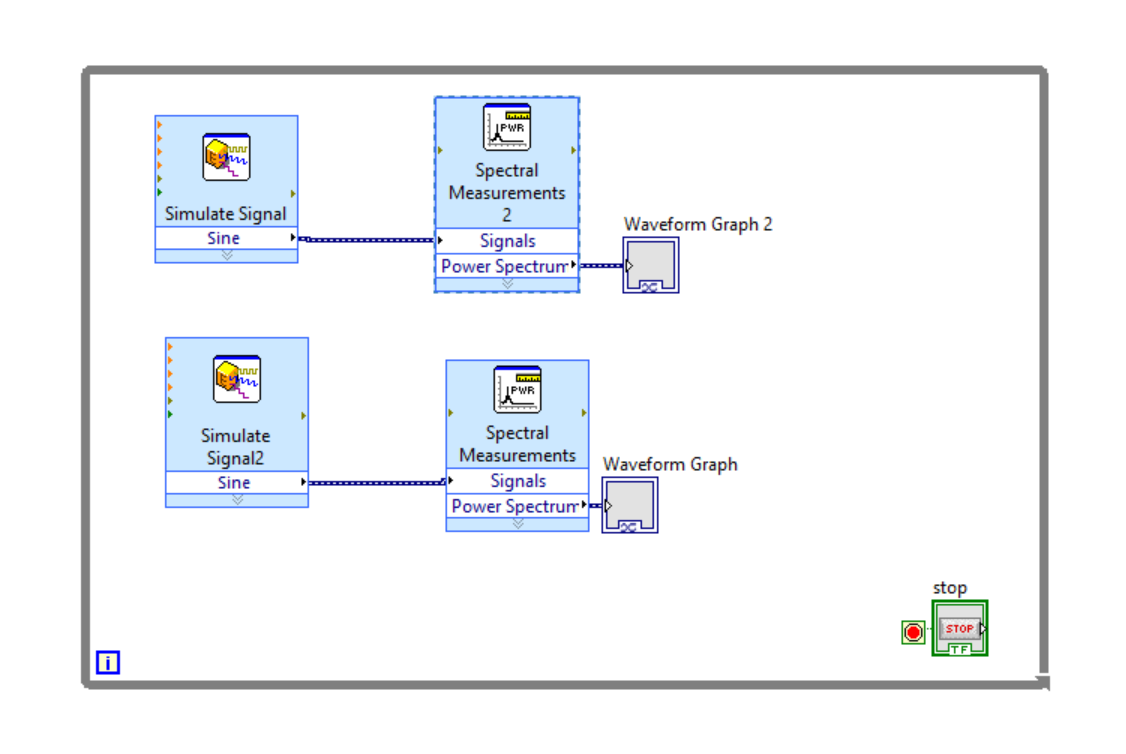
\includegraphics[width=\columnwidth]{images/05a_labview_diagrama_p1.png}
\caption{Diagrama de bloques del VI en LabVIEW (primera parte): dos \textit{Simulate Signal} (0.05~Hz/amplitud 1 y 0.25~Hz/amplitud 0.5, ambos a 20 S/s y $N=1024$) $\rightarrow$ sendos \textit{Spectral Measurements} (\textit{Power Spectrum}, resultado lineal) $\rightarrow$ \textit{Waveform Graph}, todo dentro de un \textit{While Loop} con botón \texttt{stop}.}
\label{fig:labview_diagrama_p1}
\end{figure}

\begin{figure}[!t]
\centering
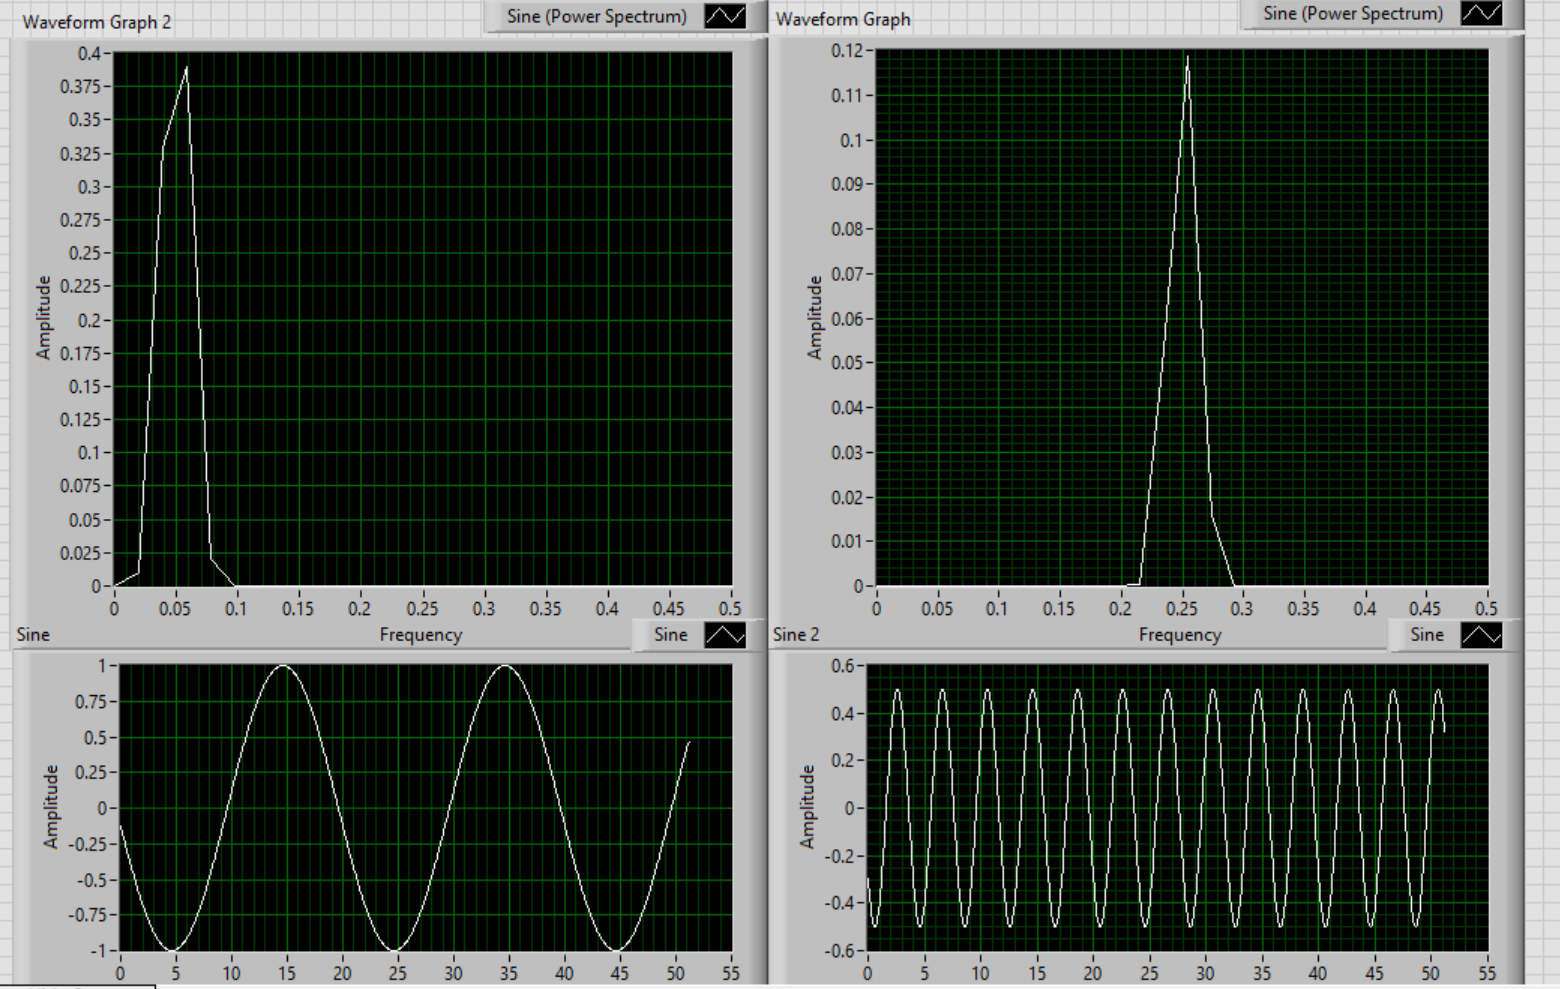
\includegraphics[width=\columnwidth]{images/05b_labview_graficas_p1.png}
\caption{Panel frontal, primera parte: espectros de potencia (arriba) y señales en el dominio del tiempo (abajo). Izquierda: componente de 0.05~Hz, amplitud temporal 1, pico espectral $\approx0.39$. Derecha: componente de 0.25~Hz, amplitud temporal 0.5, pico espectral $\approx0.12$. Ventana temporal de 51.2~s.}
\label{fig:labview_graficas_p1}
\end{figure}

Las gráficas temporales confirman los parámetros configurados: la primera señal completa aproximadamente 2.5 ciclos en la ventana de $T=N/F_s=51.2$~s (consistente con un periodo de 20~s a 0.05~Hz) oscilando entre $-1$ y $+1$, mientras que la segunda completa alrededor de 12.8 ciclos (periodo de 4~s a 0.25~Hz) oscilando entre $-0.5$ y $+0.5$. Los espectros muestran, respectivamente, un único pico en 0.05~Hz y otro en 0.25~Hz, coincidentes con las frecuencias de diseño.

\textbf{¿Cuál es la resolución espectral de este montaje?} Aplicando la ecuación \eqref{eq:resolucion} con $F_s=20$~Hz y $N=1024$:
\begin{equation}
\Delta f = \frac{F_s}{N} = \frac{20}{1024} \approx 0.01953~\text{Hz}
\label{eq:labview_res}
\end{equation}

\textbf{¿Es esta resolución suficiente para distinguir 0.05~Hz de 0.25~Hz?} Sí, ampliamente: la separación entre ambas frecuencias es de $0.25-0.05=0.20$~Hz, más de diez veces mayor que $\Delta f\approx0.0195$~Hz, por lo que ambos picos aparecerían claramente resueltos en \textit{bins} de FFT distintos y separados por varios \textit{bins} vacíos entre sí.

\textbf{¿Qué frecuencias aparecen en el espectro y coinciden con las configuradas?} Sí coinciden. Como se observa en la Figura \ref{fig:labview_graficas_p1}, el \textit{Power Spectrum} de cada señal muestra una única línea espectral bien definida, ubicada en $f\approx0.05$~Hz para el primer generador y en $f\approx0.25$~Hz para el segundo, exactamente en las frecuencias configuradas en los bloques \textit{Simulate Signal}; el resto de la banda observable (hasta $F_s/2=10$~Hz, mostrada aquí con acercamiento hasta 0.5~Hz) permanece esencialmente en cero.

\textbf{¿Por qué la componente de 0.25~Hz tiene menor magnitud que la de 0.05~Hz?} Porque su amplitud en el dominio del tiempo es menor por diseño (0.5 frente a 1); la magnitud de la línea espectral de una senoidal pura es directamente proporcional a su amplitud temporal ($|X(f_0)|\propto A$). Esto se verifica en la medición: el pico de 0.05~Hz alcanza aproximadamente 0.39 mientras que el de 0.25~Hz llega a cerca de 0.12, es decir, la componente de menor amplitud presenta un pico espectral apreciablemente menor. La razón medida ($\approx0.31$) es menor que el factor 0.5 esperado de la proporcionalidad lineal pura, lo cual se explica por la fuga espectral: al no contener la ventana un número entero de periodos de ninguna de las dos componentes, parte de la energía de cada pico se dispersa hacia \textit{bins} vecinos, y el reparto no es idéntico para ambas frecuencias (2.56 periodos frente a 12.8 periodos en la ventana), de modo que la altura del pico principal se ve atenuada en distinta proporción en cada caso.

\textbf{¿El espectro combinado muestra una línea o varias?} Al analizar cada señal por separado, cada espectro individual muestra una única línea dominante en su frecuencia respectiva (Figura \ref{fig:labview_graficas_p1}). Al sumar ambas señales antes del análisis espectral, el espectro combinado muestra dos líneas separadas, una en 0.05~Hz y otra en 0.25~Hz, y no una sola línea ensanchada, precisamente porque la separación entre ambas (0.20~Hz) excede ampliamente la resolución $\Delta f$ del montaje; este resultado se documenta experimentalmente más adelante en la Figura \ref{fig:labview_espectro_suma}.

\textbf{¿Qué parámetro afecta más la resolución espectral, $F_s$ o $N$?} De la ecuación \eqref{eq:resolucion}, $\Delta f=F_s/N$, ambos parámetros influyen, pero en direcciones opuestas: aumentar $F_s$ (a $N$ fijo) \textit{empeora} la resolución (aumenta $\Delta f$), mientras que aumentar $N$ (a $F_s$ fijo) la \textit{mejora} (reduce $\Delta f$). En la práctica, el parámetro más eficaz para mejorar la resolución es alargar la ventana de observación $T=N/F_s$, ya sea aumentando $N$ a $F_s$ constante o, equivalentemente, reduciendo $F_s$ si el contenido espectral de interés lo permite sin violar Nyquist; para este montaje, $N$ es el parámetro que el usuario ajustaría típicamente, ya que $F_s=20$~Hz está fijado por el fenómeno físico a muestrear.

\textbf{¿Qué ocurriría con $N=128$ en lugar de 1024?} La nueva resolución sería $\Delta f = 20/128 \approx 0.15625$~Hz. Esta resolución sigue siendo suficiente para distinguir 0.05~Hz de 0.25~Hz, dado que su separación (0.20~Hz) continúa siendo mayor que $\Delta f$, aunque el margen se reduce considerablemente (de un factor mayor a 10 con $N=1024$ a apenas un factor de 1.28 con $N=128$), y los picos resultarían visiblemente más anchos, con mayor riesgo de solaparse si las frecuencias estuviesen ligeramente más próximas entre sí o si existiera fuga espectral apreciable por una ventana no entera en periodos.

\textbf{Segundo escenario: ¿qué ocurre al reducir el \textit{sample rate} a 0.3~S/s?} La guía propone reconfigurar ambos bloques \textit{Simulate Signal} a 0.3 muestras por segundo, manteniendo $N=1024$, para provocar aliasing sobre la componente de 0.25~Hz. \textbf{Este valor no pudo introducirse}: el Express VI \textit{Simulate Signal} rechazó la configuración con un error indicando que la tasa de muestreo debe ser al menos el doble de la frecuencia de la señal. El resultado experimental más significativo de esta parte del ejercicio es, por tanto, el propio rechazo del software.

La razón es exactamente la condición de Nyquist: para la señal de 0.25~Hz se exige $F_s>2f_{\text{señal}}=0.5$~Hz, y $0.3$~S/s no la satisface. LabVIEW valida este criterio \emph{a priori}, en el diálogo de configuración del Express VI, en lugar de permitir la adquisición y entregar después un espectro corrupto: al generar internamente la señal a partir de su descripción analítica, el bloque conoce de antemano la frecuencia que se le pide sintetizar y puede comprobar la desigualdad antes de producir una sola muestra. El comportamiento contrasta con el de un sistema de adquisición real conectado a una señal física desconocida, donde nada impide muestrear por debajo de Nyquist y el aliasing solo se descubre \emph{a posteriori}, al observar picos espectrales en frecuencias donde no debería haber energía; es precisamente por ello que los sistemas de adquisición reales incorporan un filtro anti-aliasing analógico antes del convertidor A/D, que elimina físicamente el contenido por encima de $F_s/2$ y hace imposible el repliegue.

Analíticamente, de haberse podido ejecutar la configuración, la frecuencia de Nyquist habría sido $F_s/2=0.15$~Hz, muy por debajo de la componente de 0.25~Hz, la cual se habría replegado (\textit{alias}) hacia una frecuencia falsa dentro de la banda base observable, $f_{\text{alias}}=|f_{\text{señal}}-F_s\cdot\text{round}(f_{\text{señal}}/F_s)|=|0.25-0.3|=0.05$~Hz, resultando indistinguible en el espectro de la componente genuina de 0.05~Hz.

\textbf{Escenario efectivamente ejecutado: $F_s=0.5$~S/s.} Para documentar experimentalmente la degradación se empleó el menor valor que el bloque aceptó, $F_s=0.5$~S/s, es decir, exactamente el límite de Nyquist para la componente de 0.25~Hz ($F_s=2f_{\text{señal}}$, la frontera del criterio, que exige desigualdad estricta). El resultado se muestra en la Figura \ref{fig:labview_aliasing}.

\begin{figure}[!t]
\centering
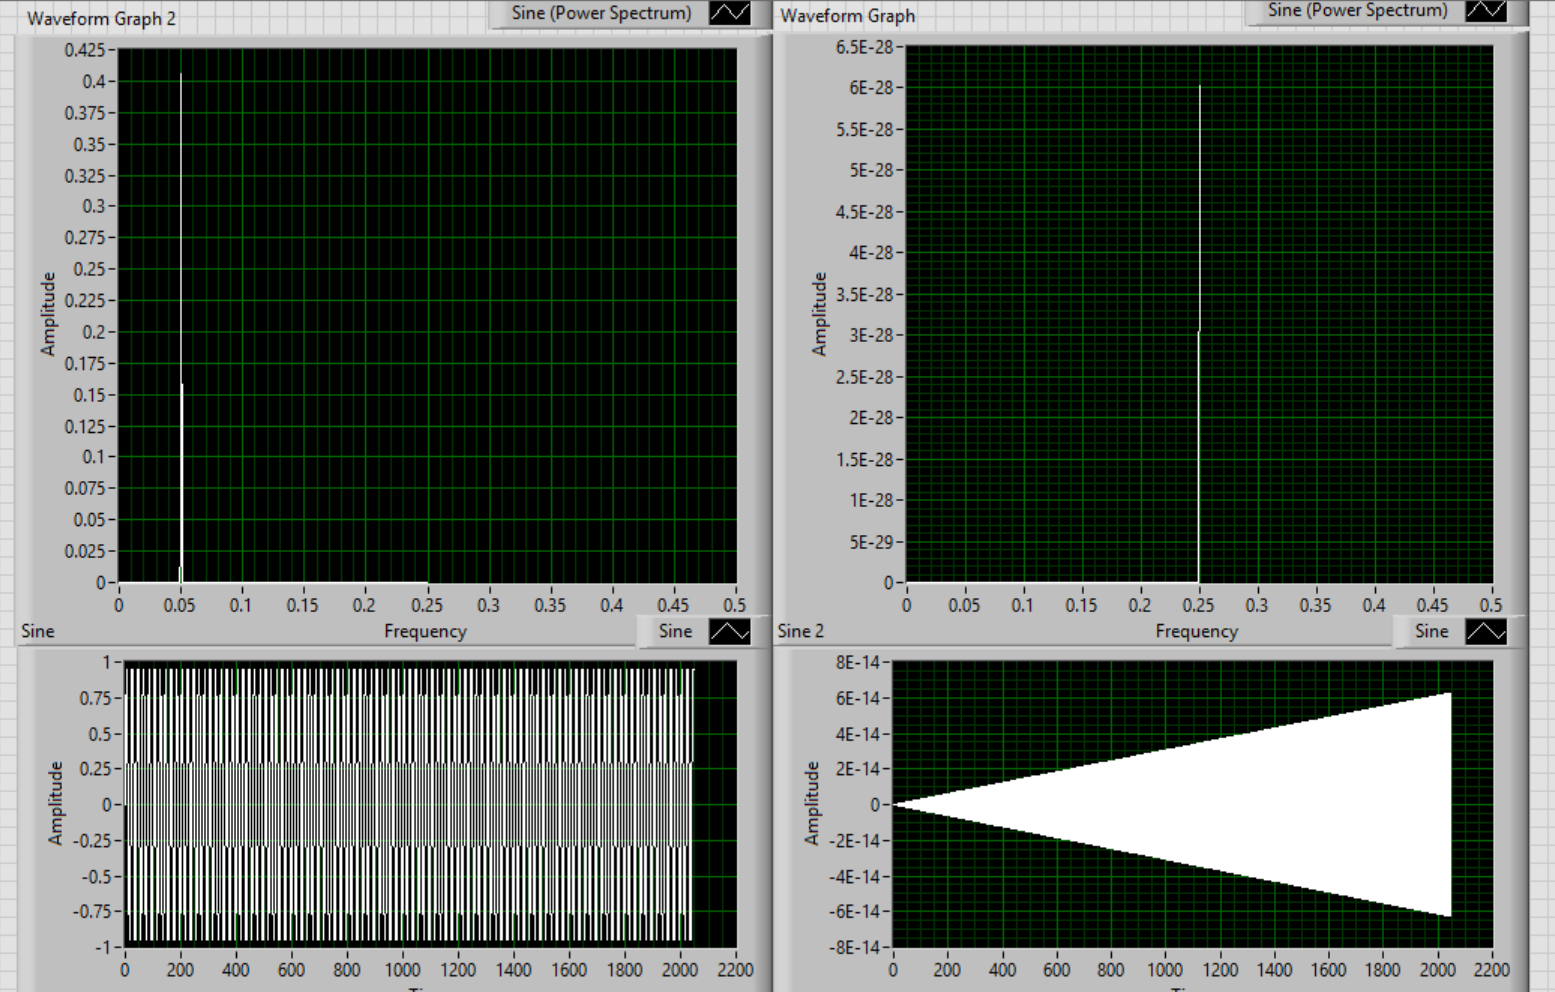
\includegraphics[width=\columnwidth]{images/05c_labview_aliasing.png}
\caption{Muestreo en el límite de Nyquist ($F_s=0.5$~S/s, $N=1024$): espectros de potencia (arriba) y señales temporales (abajo). La ventana se extiende a $T=2048$~s; la señal de 0.05~Hz (izq.) aparece como una banda densamente oscilante por la compresión del eje temporal, conservando su pico espectral en 0.05~Hz, mientras que la de 0.25~Hz (der.), muestreada exactamente a $2f$, colapsa a una amplitud de orden $10^{-14}$ y a un pico espectral de orden $10^{-28}$, ambos residuo numérico sin significado físico.}
\label{fig:labview_aliasing}
\end{figure}

El comportamiento de ambas señales difiere radicalmente. La ventana de observación se extiende de 51.2~s a $T=N/F_s=1024/0.5=2048$~s, por lo que las gráficas temporales comprimen ahora más de 100 periodos de la primera señal y la muestran como una banda densamente oscilante; aun así, la componente de 0.05~Hz sigue cumpliendo Nyquist con holgura ($0.5>2\times0.05=0.1$) y su pico espectral permanece correctamente ubicado en 0.05~Hz, con magnitud comparable a la del montaje original.

La componente de 0.25~Hz, en cambio, desaparece: su amplitud temporal cae al orden de $10^{-14}$ y su pico espectral al orden de $10^{-28}$, valores que no representan energía real sino residuo numérico de punto flotante. La causa es que $F_s=0.5$~S/s equivale a muestrear esta señal exactamente a $2f$, es decir, justo dos muestras por periodo, sobre la frontera del criterio de Nyquist, que exige desigualdad estricta ($F_s>2f$) precisamente para excluir este caso. Al muestrear una senoidal $\sin(2\pi f t)$ en instantes $t_n=n/(2f)$, todas las muestras caen sobre los cruces por cero de la onda y el resultado teórico es idénticamente nulo: la señal reconstruida es la señal cero, y el $10^{-14}$ observado es únicamente el error de redondeo de la aritmética de punto flotante al evaluar senos de múltiplos de $\pi$. Este resultado ilustra por qué el teorema de muestreo se enuncia con desigualdad estricta y no con $\geq$: muestrear exactamente al doble de la frecuencia no basta, ya que la información de fase y amplitud puede perderse íntegramente según dónde caigan las muestras.

En síntesis, la tasa de 0.3~S/s propuesta por la guía es insuficiente para representar la señal de 0.25~Hz y el propio software lo impide; la tasa mínima admisible, 0.5~S/s, tampoco la representa, por situarse justo sobre la frontera del criterio. La condición general que debe cumplirse es que la frecuencia de muestreo supere estrictamente el doble de la componente de mayor frecuencia presente en la señal ($F_s>2f_{max}$), en la práctica con margen adicional apreciable (habitualmente $F_s\geq5f_{max}$ o más, como los $10\,000$~Hz empleados frente a los 360~Hz del Ejercicio 3) tanto para facilitar el filtrado anti-aliasing como para obtener una representación temporal visualmente fiel de la forma de onda.

\textbf{¿Qué representa físicamente el \textit{Power Spectrum}?} El \textit{Power Spectrum} representa la distribución de la potencia (energía por unidad de tiempo) de la señal en función de la frecuencia, es decir, cuánta potencia aporta cada componente espectral al contenido total de la señal; mientras que la FFT simple entrega una magnitud/fase compleja por \textit{bin}, el \textit{Power Spectrum} típicamente reporta el cuadrado de dicha magnitud (proporcional a la potencia, según el teorema de Parseval), por lo que es la herramienta natural para cuantificar cuánta energía transporta cada frecuencia presente en una señal.

\textbf{¿Por qué una mayor amplitud genera mayor energía, y cómo se relaciona la amplitud en el tiempo con la magnitud espectral?} La energía (o potencia promedio) de una señal senoidal es proporcional al cuadrado de su amplitud ($P\propto A^2/2$); dado que la FFT es una transformación lineal, la magnitud del \textit{bin} espectral correspondiente también es directamente proporcional a la amplitud temporal de la componente ($|X(f_0)|\propto A$), y por lo tanto la potencia en ese \textit{bin} (magnitud al cuadrado) es proporcional a $A^2$. Esto explica numéricamente por qué la componente de 0.25~Hz (amplitud 0.5) exhibe una magnitud espectral igual a la mitad de la de 0.05~Hz (amplitud 1), y una potencia igual a un cuarto.

\textbf{¿Qué sucede si se duplica la amplitud de la señal de 0.25~Hz (de 0.5 a 1.0)?} Por la linealidad de la FFT, la magnitud de la línea espectral en 0.25~Hz se duplicaría también, igualándose a la de la componente de 0.05~Hz, mientras que la potencia asociada (magnitud al cuadrado) se cuadriplicaría; ninguna otra línea del espectro se vería afectada, ya que la operación no introduce nuevas componentes frecuenciales.

\textbf{Si se suman ambas señales antes de la FFT, ¿cómo se ve el espectro combinado, interfieren las frecuencias, y qué principio matemático lo explica?} Para responder experimentalmente esta pregunta se amplió el VI (Figura \ref{fig:labview_diagrama_suma}) añadiendo una función \texttt{Add} que suma las dos salidas \textit{Sine} y un tercer \textit{Spectral Measurements} con su correspondiente \textit{Waveform Graph}, alcanzando así las seis gráficas solicitadas por la guía. El espectro combinado medido (Figura \ref{fig:labview_espectro_suma}) muestra dos picos claramente separados e independientes: uno en $\approx0.05$~Hz con magnitud $\approx0.39$ y otro en $\approx0.25$~Hz con magnitud $\approx0.12$, es decir, exactamente las mismas posiciones y alturas que exhibían los espectros individuales de la Figura \ref{fig:labview_graficas_p1}, sin líneas adicionales entre ellos ni desplazamiento alguno de los picos originales.

\begin{figure}[!t]
\centering
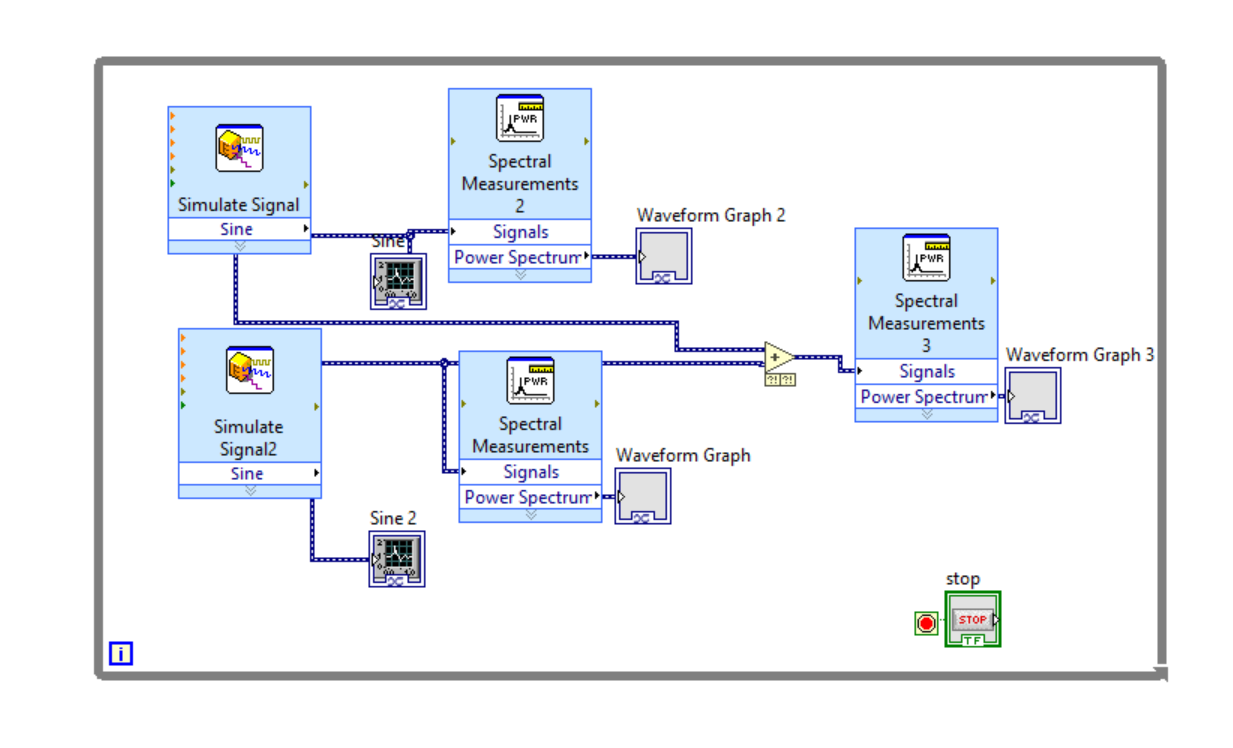
\includegraphics[width=\columnwidth]{images/05d_labview_diagrama_suma.png}
\caption{Diagrama de bloques ampliado: las dos salidas \textit{Sine} se suman mediante la función \texttt{Add} y alimentan un tercer \textit{Spectral Measurements} (\textit{Spectral Measurements 3}) cuyo \textit{Power Spectrum} se despliega en \textit{Waveform Graph 3}, completando las seis gráficas del montaje.}
\label{fig:labview_diagrama_suma}
\end{figure}

\begin{figure}[!t]
\centering
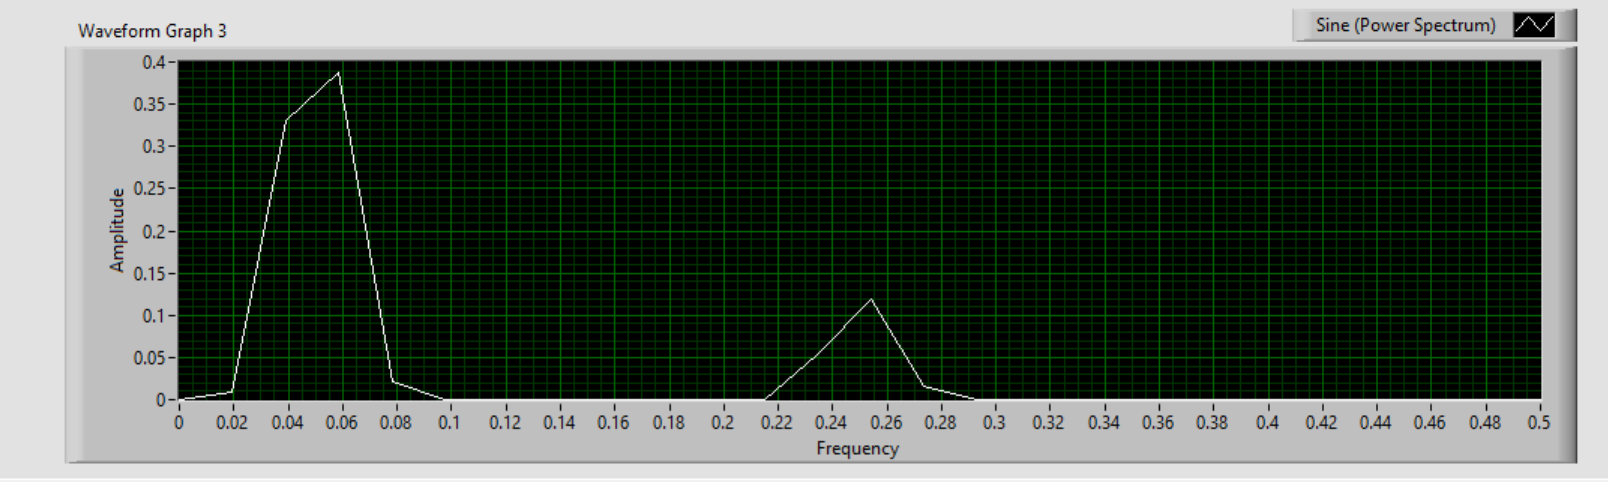
\includegraphics[width=\columnwidth]{images/05e_labview_espectro_suma.png}
\caption{Espectro de potencia de la señal suma $x(t)=x_1(t)+x_2(t)$: dos líneas independientes en 0.05~Hz (magnitud $\approx0.39$) y 0.25~Hz (magnitud $\approx0.12$), idénticas a las de los espectros individuales, confirmando la linealidad de la Transformada de Fourier.}
\label{fig:labview_espectro_suma}
\end{figure}

Este resultado confirma el principio de \textbf{linealidad} de la Transformada de Fourier: el espectro de la suma es exactamente la suma de los espectros individuales, $X(f)=X_1(f)+X_2(f)$. Como las dos frecuencias están bien resueltas (separación de 0.20~Hz frente a $\Delta f\approx0.0195$~Hz), ambas componentes coexisten en el espectro sin mezclarse ni interferir entre sí en el dominio de la frecuencia; no se crean componentes nuevas ni modulación cruzada, porque el sistema (suma más FFT) es lineal. Escalar o sumar señales de entrada produce el escalamiento o la suma correspondiente en la salida espectral, sin términos cruzados adicionales, lo cual sí ocurriría, por ejemplo, si las señales se multiplicaran en lugar de sumarse, generando productos de intermodulación.

\textbf{¿Qué es el \textit{spectral leakage} y cómo influye la ventana temporal en la FFT?} Si la señal analizada no es periódica dentro de la ventana de observación (es decir, si la ventana de $N$ muestras no contiene un número entero de periodos de cada componente), la FFT —que asume implícitamente que la señal se repite periódicamente fuera de la ventana— introduce una discontinuidad artificial en los bordes; esta discontinuidad dispersa la energía de cada componente pura hacia \textit{bins} vecinos en lugar de concentrarla en un único \textit{bin}, fenómeno conocido como fuga espectral (\textit{spectral leakage}). El resultado es un pico principal más ancho y de menor amplitud aparente, junto con lóbulos laterales espurios que pueden enmascarar componentes débiles cercanas. Con $F_s=20$~Hz y $N=1024$, la ventana dura $T=N/F_s=51.2$~s; dado que el periodo de la señal de 0.05~Hz es $1/0.05=20$~s y el de 0.25~Hz es $1/0.25=4$~s, la ventana contiene 2.56 periodos de la primera componente (no entero) y 12.8 periodos de la segunda (tampoco entero), por lo que cabe esperar cierto grado de fuga espectral en ambas líneas. Los resultados medidos lo confirman: los picos de las Figuras \ref{fig:labview_graficas_p1} y \ref{fig:labview_espectro_suma} no aparecen como líneas de un solo \textit{bin}, sino como lóbulos de anchura apreciable (aproximadamente 0.04~Hz de base en el pico de 0.05~Hz y algo menos en el de 0.25~Hz, frente a un $\Delta f$ de apenas 0.0195~Hz), y sus alturas resultan atenuadas respecto a la proporcionalidad lineal exacta con la amplitud temporal, como se discutió anteriormente. Aun así, la separación entre ambas componentes es más que suficiente para distinguirlas sin ambigüedad.

\textbf{¿Qué tipo de ventana reduciría el \textit{leakage}?} Ventanas de suavizado (\textit{tapering windows}) como Hann, Hamming o Blackman, que atenúan gradualmente la señal hacia cero en los bordes de la ventana de observación en lugar de truncarla abruptamente, reducen la discontinuidad artificial y, con ella, la energía dispersada hacia \textit{bins} vecinos, a cambio de ensanchar ligeramente el lóbulo principal (compromiso resolución-\textit{leakage} inherente a toda ventana no rectangular).

\textbf{¿Por qué la FFT es más eficiente que la DFT directa?} La Transformada Discreta de Fourier (DFT) calculada directamente a partir de su definición requiere, para $N$ muestras, del orden de $O(N^2)$ operaciones (cada uno de los $N$ coeficientes de salida es una suma de $N$ términos). La Transformada Rápida de Fourier (FFT) explota la redundancia y las simetrías de las raíces de la unidad para calcular el mismo resultado en $O(N\log_2 N)$ operaciones, mediante un esquema de divide y vencerás (por ejemplo, el algoritmo de Cooley-Tukey) que descompone recursivamente la DFT de $N$ puntos en DFTs más pequeñas \cite{proakis}. Para $N=1024=2^{10}$, esto representa una reducción de aproximadamente $N^2/(N\log_2 N)=N/\log_2 N=1024/10\approx102$ veces menos operaciones que la DFT directa, una diferencia que se vuelve crítica para el procesamiento en tiempo real de señales con miles o millones de muestras.

\textbf{¿Dónde se usa este tipo de análisis espectral en telecomunicaciones?} El análisis de \textit{Power Spectrum}/FFT descrito en este ejercicio tiene aplicaciones directas en telecomunicaciones e ingeniería relacionada: (i) \textit{detección de interferencia}, identificando portadoras o señales espurias no deseadas dentro de una banda de operación al observar picos en frecuencias no esperadas del espectro monitoreado; (ii) \textit{ruido armónico en la red eléctrica}, aplicando exactamente el mismo principio empleado en el Ejercicio 3 de este informe (Sección VI) para cuantificar el contenido de armónicos de 60~Hz y su THD mediante picos espectrales; (iii) \textit{detección de vibraciones anormales en motores}, donde acelerómetros o sensores de vibración alimentan un análisis espectral similar para identificar frecuencias características de fallas mecánicas (desbalance, desalineación, defectos de rodamiento), cada una asociada a una banda de frecuencia característica en función de la velocidad de rotación; y (iv) para \textit{señales de audio}, el parámetro que cambiaría más significativamente es la frecuencia de muestreo $F_s$, que debe elevarse hasta al menos el doble del ancho de banda audible (típicamente $F_s=44\,100$~Hz o $48\,000$~Hz, frente al ancho de banda de audio de hasta 20~kHz), muy por encima de los 20~Hz empleados en este montaje de señales de baja frecuencia.

\section{Discusión Integrada}

Los resultados de este informe conectan cuatro niveles de análisis: el conceptual (arquitectura y numeración de la PSTN), el de señales de referencia (Ejercicio 1), el de distorsión armónica en sistemas de potencia con su vínculo a telecomunicaciones (Ejercicio 3), y el de verificación instrumental del análisis espectral (LabVIEW). En el nivel conceptual, la limitación de ancho de banda de voz a 4~kHz y el plan de numeración jerárquico NPA-NXX-Station son consecuencias directas de decisiones de ingeniería tomadas para maximizar la capacidad de la red analógica original, decisiones cuyo legado persiste incluso en redes NGN basadas en conmutación de paquetes.

En el nivel de señales de referencia, se observa un patrón recurrente: las funciones tipo $\text{Sa}$/sinc (ítems 2 y 9) están íntimamente ligadas al teorema de muestreo y a la interferencia intersímbolo; el escalón (ítem 5) y la exponencial creciente (ítem 7) modelan transitorios y comportamientos inestables de conmutación; las exponenciales complejas (ítems 3 y 4) son la base matemática de la modulación en cuadratura empleada en prácticamente todo sistema de comunicación digital moderno; y la suma de senoidales de frecuencias no relacionadas armónicamente (ítem 12) anticipa, en miniatura, el fenómeno de distorsión armónica estudiado en profundidad en el Ejercicio 3.

En el nivel de distorsión armónica, el THD calculado (aproximadamente 70.1\%) para las amplitudes de diseño evidencia por qué las normas eléctricas limitan estrictamente el contenido armónico permitido, y por qué dicho contenido armónico es también relevante para telecomunicaciones: los mismos armónicos que sobrecalientan transformadores generan interferencia electromagnética de banda ancha que puede acoplarse a líneas de comunicación adyacentes (diafonía inducida por líneas de potencia), especialmente en instalaciones donde el cableado eléctrico y el de datos comparten canalizaciones. La validación mediante Simulink, con errores de frecuencia y amplitud inferiores al 2\% respecto al diseño, confirma que un modelo por bloques puede reproducir fielmente el comportamiento matemático esperado cuando los parámetros de muestreo (Nyquist, resolución, ventana entera en periodos) se seleccionan correctamente, tal como fue el caso en esta corrida particular; el análisis conceptual de las cuatro causas de error espectral (aliasing, \textit{leakage}, resolución insuficiente, configuración del analizador) sigue siendo, no obstante, un marco de diagnóstico necesario para configuraciones futuras donde dichos parámetros no se elijan con el mismo cuidado.

En el nivel instrumental, el montaje en LabVIEW cierra el ciclo al someter los mismos principios a verificación experimental en un entorno de instrumentación virtual: la resolución espectral predicha por la ecuación \eqref{eq:resolucion} se tradujo en dos picos efectivamente separados; la linealidad de la Transformada de Fourier, invocada implícitamente en todo el informe al descomponer señales compuestas en sus componentes, quedó comprobada al observar que el espectro de la suma de dos senoidales conserva intactas ambas líneas; y la fuga espectral, discutida teóricamente en la Sección III-C y listada como causa potencial de error en la Sección VI-D, se manifestó de forma medible en el ensanchamiento de los picos y en la atenuación de su altura respecto a la proporcionalidad lineal exacta con la amplitud temporal. Resulta especialmente instructivo el contraste entre el modelo Simulink, donde la ventana se eligió deliberadamente con un número entero de periodos y el espectro resultó prácticamente libre de fuga, y el montaje en LabVIEW, donde los parámetros fijados por la guía ($F_s=20$~S/s, $N=1024$) no son enteros en periodos para ninguna de las dos componentes y la fuga se hizo visible: la misma teoría explica ambos resultados, y la diferencia radica exclusivamente en la elección de los parámetros de adquisición.

El intento de reproducir el escenario de aliasing añadió una observación de carácter práctico ausente del planteamiento teórico. El criterio de Nyquist no operó aquí como una predicción sobre el resultado del experimento, sino como una restricción impuesta por el instrumento antes de permitirlo: LabVIEW rechazó la tasa de 0.3~S/s en el diálogo de configuración, y la mínima tasa aceptada anuló por completo la componente de 0.25~Hz. Esta diferencia entre validar el criterio \emph{a priori}, posible cuando la señal se sintetiza a partir de una descripción analítica conocida, y descubrir su violación \emph{a posteriori}, que es la situación habitual al digitalizar una señal física de contenido espectral desconocido, es justamente la que justifica el filtro anti-aliasing analógico que precede al convertidor A/D en todo sistema de adquisición real, y también el filtrado que limita la voz a la banda de 300--3400~Hz antes de su codificación PCM a 8000 muestras por segundo en la central telefónica, descrito en la Sección III-A. En un caso el instrumento puede negarse a muestrear mal; en el otro solo cabe garantizar, por hardware y antes de muestrear, que no exista contenido por encima de $F_s/2$ capaz de replegarse.

\section{Conclusión}

Se sintetizó el marco conceptual de la PSTN, describiendo sus componentes (centrales, red de señalización, bucle de abonado, CPE), su jerarquía de conmutación, su plan de numeración NPA-NXX-Station (ejemplificado con \texttt{234-234-5678} válido frente a \texttt{123-234-5678} inválido) y su evolución hacia redes de próxima generación basadas en \textit{softswitch} y conmutación de paquetes. Se generaron y analizaron exitosamente las doce señales analógicas de referencia del Ejercicio 1 y la señal senoidal amortiguada complementaria, documentando explícitamente los supuestos adoptados ante las ambigüedades de los ítems 1, 2, 7, 9 y 12, e interpretando cada señal tanto en su naturaleza física (o su carácter de función matemática abstracta, como en los ítems 2, 7, 9 y 10) como en su aplicación análoga en sistemas de telecomunicaciones reales.

El Ejercicio 3 modeló una señal eléctrica de 60~Hz con cinco armónicos adicionales (THD calculado de aproximadamente 70.1\%), validando el modelo mediante un análisis FFT en MATLAB y un modelo equivalente en Simulink. La comparación de los seis picos espectrales detectados automáticamente contra los valores de diseño mostró errores de frecuencia inferiores a 0.06~Hz y errores de amplitud inferiores al 2\% en todos los casos, confirmando que, para la configuración de muestreo empleada ($F_s=10\,000$~Hz, ventana de 0.1~s con seis periodos exactos de la fundamental), el espectro obtenido en Simulink coincidió con el esperado y no exhibió síntomas de aliasing ni de fuga espectral significativa; la discusión de las cuatro causas típicas de error espectral se presentó como respuesta conceptual a la pregunta genérica del enunciado, aplicable a configuraciones distintas a la aquí documentada.

Finalmente, se implementó y ejecutó en LabVIEW el ejercicio de análisis espectral propuesto en la guía. Con $N=1024$ muestras a $F_s=20$~S/s (resolución espectral $\Delta f\approx0.0195$~Hz), los espectros de potencia medidos ubicaron sendas líneas en 0.05~Hz y 0.25~Hz, coincidentes con las frecuencias configuradas y holgadamente resueltas entre sí, con magnitudes de aproximadamente 0.39 y 0.12 que reflejan la diferencia de amplitud temporal (1 frente a 0.5) atenuada por la fuga espectral inherente a una ventana que no contiene un número entero de periodos de ninguna de las dos componentes. Al sumar ambas señales antes del análisis espectral, el espectro combinado mostró las dos líneas independientes en sus posiciones y magnitudes originales, verificando experimentalmente la linealidad de la Transformada de Fourier, y el ejercicio de submuestreo arrojó un resultado no anticipado por el enunciado: la tasa de 0.3~S/s solicitada por la guía no pudo configurarse, pues el Express VI \textit{Simulate Signal} valida el criterio de Nyquist en su propio diálogo y rechaza toda tasa inferior al doble de la frecuencia sintetizada. Empleando la mínima tasa admitida (0.5~S/s), exactamente $2f$ para la componente de 0.25~Hz, dicha componente se anuló hasta el nivel del residuo numérico de punto flotante ($\sim10^{-14}$), al caer todas sus muestras sobre los cruces por cero de la onda, mientras que la componente de 0.05~Hz, que sí conserva holgura respecto a Nyquist, se mantuvo correctamente ubicada en el espectro. Este resultado ilustra de forma directa por qué el teorema de muestreo se enuncia con desigualdad estricta ($F_s>2f_{max}$) y no con $\geq$. Se explicó además el rol regulatorio complementario de la FCC (regulación nacional en EE.~UU.) y la ITU (armonización de estándares y espectro a escala global), y se resumieron los principales tipos de cableado empleados en redes de telecomunicaciones y datos.

\bibliographystyle{IEEEtran}
\bibliography{references}

\end{document}
